\chapter{Konzeption}
Die im vorherigen Abschnitt dargelegten Probleme, Motivationen und Anforderungen werden im folgenden Kapitel in ein Lösungskonzept gefasst. Dieses Lösungskonzept schlägt vor, beschreibt, analysiert und rationalisiert ein Programmierungskonzept, einzelnen Komponenten sowie deren Darstellungsform.

\section{Rationale}\label{sec:einleitungkonzept}
Im Folgenden werden grundsätzliche Entscheidungen für die Gestaltung des \ac{EUD}-Kon\-zepts auf Basis der Anforderungen getroffen. Zu diesem Zweck werden diese Entscheidungsalternativen aufgezählt, beschrieben und auf Basis ihrer Vor- und Nachteile ausgewählt und begründet.

\subsection{Optionen}\label{subsec:optionen}
In den vorherigen Kapiteln (Sektion \ref{subsec:stateoftheart} u. Kapitel \ref{chapter:analyse}) wurden die Qualitäten/eigenschaften von bestehenden \ac{EUD}-Lösungen in Form von Darstellung und Programmierparadigma diskutiert, sowie die Probleme und Anforderungen, die an das Projekt gestellt werden, analysiert. Aus der folgenden Arbeit resultieren zwei grundlegende Entscheidungen, die für das Konzept getroffen werden: die \textbf{Darstellungsform} des Programmcodes und das \textbf{Programmierparadigma} selbst. 

Für die Darstellungsform der Programmlogik innerhalb der \ac{EUD} kommen zwei Optionen in Frage:
\paragraph{Textuelle Darstellung} Hierunter zählen viele \textit{general-purpose} Programmiersprachen wie C, Java, etc. und spezifische \acp{DSL}. Instruktionen zur Verarbeitung von Informationen werden hierbei in einem Fließtext gespeichert bzw. dargestellt. Generische Programmiersprachen besitzen einen sehr hohen Abstraktionsgrad, da sie prinzipiell von ihrem Anwendungsdomäne losgelöst sind. \acp{DSL} sind wie der Name suggeriert vom Abstraktionsgrad wesentlich näher an der Anwendungsdomäne. Sie bilden einen Kompromiss zwischen Erlernbarkeit und Umfang der Anwendbarkeit \cite{green1991comprehensibility}.

\paragraph{Graphische Darstellung} In dieser Darstellungsform werden Programme durch Manipulation von graphischen Elementen und Symbolen erstellt. Durch die Verwendung von graphischen Elementen wird versucht eine Metapher zwischen der physischen Welt und der digitalen Welt zu erstellen. Die Anwendungsbereiche sind vielfältig; sie reichen von Pädagogik (z.B. Scratch) zu domänenspezifische Anwendungen (z.B. SAM Studio) zu \textit{general-purpose} Anwendung (z.B. Node-RED oder DRAKON). 

Aus den vorherigen Kapiteln haben sich zwei Programmierparadigmen im \ac{EUD} für \ac{IoT} als besonders relevant hervorgetan:

\paragraph{Regeln-basiert} Das Paradigma der Regeln-basierte Programmierung manifestiert sich in Form von \ac{TAP}. Hierbei werden eintreffende Signale, mit einem Datensatz von natürlich-sprachliche Regeln, auf ihre Wahrheit geprüft. Erfüllung der Regeln führen zur Erzeugung neuer Signale oder dem Auslösen von Aktionen. 
\paragraph{Datenfluss-basiert} Anders als bei Kontrollfluss-Paradigmen, wird hierbei ein Programm nicht als ein Set von Instruktionen angesehen, die sequentiell auf einen Satz von zentral gespeicherten Daten angewandt werden (\textit{Data at rest}/von Neumann Architektur), sondern die Daten selbst werden durch einen Graphen von statischen Instruktionen geleitet (\textit{Data in motion}). Funktionen, welche die Daten transformieren sind dabei \textit{Black Boxen}, welche sobald an sämtlichen Schnittstellen Daten anliegen, diese verarbeiten. Dieses Verhalten macht Datenfluss-basierte Programmierung, im Vergleich zu Kontrollfluss-Paradigmen inhärent asynchron und parallel \cite{johnston2004advances}.

\subsection{Beurteilung}
Im Anbetracht der Stakeholder, Anforderungen und Zielsetzung des Projekts werden im Folgenden die Vor- und Nachteile der jeweiligen Optionen aus Kapitel \ref{subsec:optionen} gegeneinander Abgewogen, um einen grundlegenden Konsens für das \ac{EUD}-Konzept fest zu legen.

Textuelle Darstellung ist aus gutem Grund, eine der am weit verbreitetsten Darstellungsformen von Programmcode. Dies hat vielerlei Gründe: zuallererst spricht für eine textuelle Darstellung die Informationsdichte und Deskriptivität von geschriebenen Sprachen. Mit nur wenigen Zeichen, lassen sich komplexe Konstrukte und Verhalten beschreiben. Ausdrücke wie ''\textit{Abstract}'' sind schwer visuell eindeutig darzustellen.  Gleichzeitig bedeutet diese Ausdrucksstärke aber auch, dass dem Benutzer das Erlernen eines großen, abstrakten Vokabulars zumutbar sein muss. Zusätzlich muss hier darauf hingewiesen werden, dass die Ausdrucksstärke von textuellen Programmcode immer von den Fähigkeiten und dem mentalen Modell des Entwicklers abhängig ist. Diese Eigenschaften decken sich nicht mit den Fähigkeiten von Laura.

Über Intuitivität und Flexibilität textueller Darstellung lässt sich nur schwer Pauschalisieren. Die Darstellung von parallelem Programmcode stellt sich allerdings als besondere Herausforderung dar. Solange Programmcode sequentiell ausgeführt wird, ist die kognitive Anstrengung für den Entwickler vergleichsweise gering; von links nach rechts von oben nach unten wird der Programmcode, wie beim manuellen Lesen, ausgeführt. Simultane, mehrschichtige Ausführung von parallelem Programmcode hingegen, entspricht nicht der Metapher des sequentiellen Lesens. Hierbei leisten multidimensionale graphische Darstellungen Hilfestellung für den Benutzer. Graphische Oberflächen haben allerdings noch weitere Vorteile: im Kontext von domänenspezifischer Softwareentwicklung können sie wie \acp{DSL} durch (visuelle) Metaphern leichter, Brücken zum Anwendungskontext, schlagen. Diese domänenspezifischer Darstellung ermöglicht es Domänenexperten, die nur wenig Erfahrung mit Programmierung haben, ihr Wissen trotzdem auf die virtuelle Welt zu übertragen. Diese Theorie wird dadurch gestützt, dass die erfolgreichsten visuellen Programmiersprachen (LabVIEW, vvvvv, etc.) stark in ihrer Darstellung mit der Anwendungsdomäne gekoppelt sind und klar abgesteckten Rahmenbedingungen hinsichtlich Funktionalität besitzen. Auch Kritik gibt es gegenüber visueller Darstellung von Programmcode. Das \textit{Deutsch-Limit} nach [\cite{begel1996logoblocks}] besagt, dass es kaum möglich ist mehr als 50 Elemente gleichzeitig auf einem Bildschirm anzuzeigen, ohne die Übersicht zu verlieren. Bei einer textuellen Darstellung ist dieses Limit aufgrund der großen Informationsdichte wesentlich höher.

Die Diskussion über Datenfluss-basierter und Regeln-basierter Programmierparadigmen wurde schon an anderer Stelle geführt. Stellvertretend für beide Paradigmen können die Vor- und Nachteile von IFTTT und SAM Studio in Kapitel \ref{sec:loesungsans} bzw. die Probleme dieser Ansätze in Kapitel \ref{sec:problemanalyse} nachgelesen werden. Grundsätzlich ist zu sagen, dass der größte Vorteil von Regel-basierten Paradigmen die intuitive Natürlichsprachligkeit der Programmierung. Nachteile beinhalten mangelnde Übersicht bei großen Mengen an Regeln, Diskrepanzen bei der genauen Deutung der Regel durch Endnutzer und mangelnde Ausdrucksfähigkeit von Regeln mit komplexen Sachverhalten. Auf der anderen Seite basieren Datenfluss-Paradigmen ebenso auf einer soliden, für den End-Nutzer visualisierbaren Metapher. Dies zeigt sich in der Nutzung des Paradigmas in vielen Werkzeugen mit denen Endnutzer ohne Erfahrung in Softwareentwicklung produktiv arbeiten müssen: vvvv\footnote{\url{https://vvvv.org/} -- besucht August 2018} (für Designer), LabVIEW\footnote{\url{http://www.ni.com/de-de/shop/labview.html} -- besucht August 2018} (für Mathematiker u. Elektronikingenieure), unreal blueprint\footnote{\url{https://docs.unrealengine.com/en-us/Engine/Blueprints} -- besucht August 2018} (für Spieledesigner), etc.\,. Der Fokus auf Daten und ihre Transformation ist eine Parallele zwischen Datenfluss-Programmierung und der Charakteristiken der \ac{IoT} bzw. \textit{Smart Devices}. Dies ist ein Grund für die Verbreitung des Paradigmas in dieser Domäne. Nachteilig ist die erhöhte Komplexität im Vergleich zu Regeln-basierten Ansätzen und der hiermit verbundene Lernaufwand für den Endnutzer.

\subsection{Entscheidung}
Es ist aus der Diskussion ersichtlich, dass es schwierig eine klare Entscheidung für Programmierparadigma und Darstellung des Programmcodes zu treffen. Es gibt viele weitere Vor- und Nachteile die man noch vortragen könnte, man muss allerdings bedenken, dass die Effektivität einer solchen Entscheidung hinsichtlich Benutzerfreundlichkeit/Erlernbarkeit/etc. sich erst \textit{a posteriori} beurteilen lässt. Dies hat auch damit zu tun, dass jede \ac{EUD} speziell für ein Szenario konzipiert wird und es somit nur wenige vergleichbare Arbeiten bzw. Erprobungen in \ac{IoT}-Bereich der \acp{EUD} gibt. Nichtsdestotrotz, wird sich an dieser Stelle für eine Datenflussparadigma mit graphischer Darstellung als \ac{EUD} für flowws festgelegt. Die Punkte die für die Wahl ausschlaggebend sind:
\begin{itemize}
    \item \textbf{Graphische Darstellung} Es gibt viele Werkzeuge wie vvvv oder Scratch die schon jetzt von Designern und anderen Endnutzern verwendet werden, um in anderen Domänen, visuell zu Programmieren. Die graphische Darstellung hilft durch geeignete Metaphern, die Domäne mit dem Programmcode zu verbinden und unterstützt dabei die visuelle Denkweise von Stakeholdern wie Laura ohne sie mit abstrakten Konstrukten zu belasten. Es wird sich dadurch erhofft, die Erlernbarkeit zu fördern (siehe \hyperref[tab:NFA2]{NFA\#2}).
    \item \textbf{Graphische Darstellung} Zum digitalen Entwickeln von Prototypen in flowws, werden die physischen cBlocks benötigt. Es ist somit naheliegend, dass man die Visualität der Realität auf die virtuellen Repräsentation abbildet. flowws soll durch diese Darstellung der Elemente,  die kognitive Last von Laura reduzieren. Diese Bindung von physischem und virtuellen Zustand soll die Anforderung  \hyperref[tab:NFA1]{NFA\#1} erfüllen.
    \item \textbf{Datenfluss-Paradigma} Das Datenfluss-Paradigma ist schwerer zu erlernen wie das natürlichsprachige Regeln-basierte Paradigma. Allerdings ist die Metapher näher an der Realität. Auf elektrotechnischer Ebene wandeln cBlocks physische Phänomene in digitale Signale um, transformieren sie in eine verwendbare Form und wandeln durch Aktoren diese Signale wiederum in physikalische Phänomene um. Dieser Datenfluss auf Basis von elektrischen Signalen kann effizient durch ein Datenfluss-Paradigma auf Programmcode-Ebene emuliert werden. Es wird sich davon versprochen, die Benutzbarkeit von flowws zu verbessern und die kognitive Dissonanz zwischen Elektro- und Informatikebene zu mindern.
    \item \textbf{Datenfluss-Paradigma} Datenflüsse lassen sich gut visualisieren und  geht deshalb Hand-in-Hand mit der graphischen Darstellung des Programmcodes. Dies kommt der Benutzerfreundlichkeit und Fehleridentifikation zu Gute. Durch das Paradigma und dessen Visualisierung wird sich erhofft, Parallelität leichter begreifbar zu machen (siehe \hyperref[tab:NFA0]{NFA\#0}).
\end{itemize}

Aus diesen Gründen wurde sich für eine \ac{EUD} mit graphischer Programmierung auf Basis des Datenflussparadigmas festgelegt.

\section{Programmiermodel}
In diesem Kapitel wird sich der Konzeption eines Programmiermodells auf Basis der Anforderungen (insbesondere \hyperref[tab:NFA0]{NFA\#0}) und der Entscheidungen aus dem vorhergegangenen Kapitel erstellt.

\subsection{Datenfluss-basierte Programmierung}\label{subsection:datenflussprog}
Prototypen, die mit cBlocks entwickelt werden essentiell ein Netzwerk von Sensoren, welche Daten versenden, diese in eine nutzbare Form verwandeln und von Aktoren konsumiert werden. Sie verhalten sich so, wie die in Kapitel \ref{subsec:characIot} beschriebenen \acp{WSAN}. Diese Form von Signal-Kommunikation ist ähnlich derer von \ac{DBP}. Die Definition  laut \cite{sousa2012dataflow} von \ac{DBP} ist:
\begin{quote}
    ''\textit{Die Programmierung anhand von Datenflüssen führt ein ein neues Paradigma ein, bei dem die interne Struktur eines Programmes mit einem gerichteten Graphen repräsentiert wird, ähnlich wie bei einem Datenflussdiagramm.} ''
\end{quote}

\begin{figure}[h]
\centering
\begin{subfigure}{.45\textwidth}
  \centering
  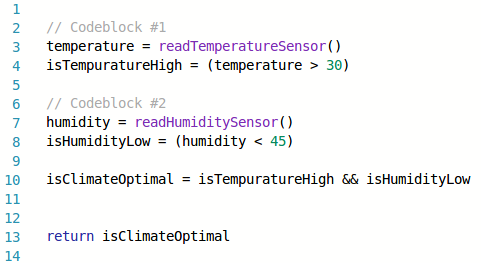
\includegraphics[width=1\linewidth]{bilder/chapter4/chapter4_2/codekbpbeispiel.png}
  \caption{}
  \label{fig:subvgldbptexttext}
\end{subfigure}%
\begin{subfigure}{.55\textwidth}
  \centering
  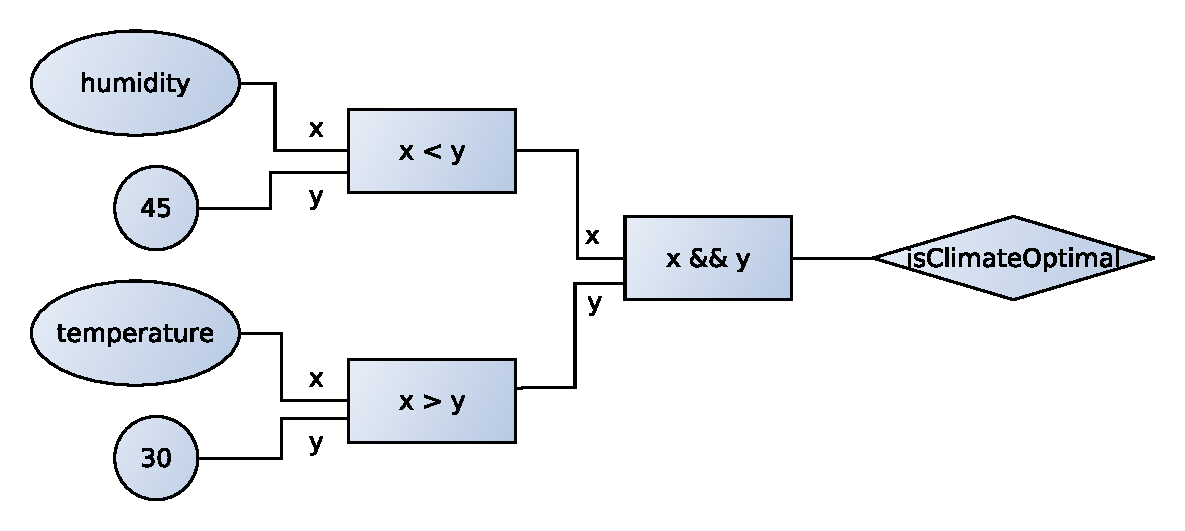
\includegraphics[width=1\linewidth]{bilder/chapter4/chapter4_2/beispieldatenfluss.pdf}
  \caption{}
  \label{fig:subvgldbptextdbp}
\end{subfigure}
    \caption{Der gleiche Programmcode in zwei Ansichten: \ac{KBP} (a) und \ac{DBP} (b). Hierbei ist die sequentielle Durchführung des \ac{KBP}-Modells mit der Parallelen des \ac{DBP} erkenntlich. Während beim linken Paradigma sequentiell die Blöcke abgearbeitet werden (wobei \#1 fertig sein muss um \#2 zu berechnen), ist das rechte Paradigma unabhängig von der Reihenfolge, in der die Signale eintreffen. Dies spiegelt den asynchronen Sachverhalt von \ac{WSAN} wieder.}
    \label{fig:bfd}
\end{figure}


Ein solches Programm wird in Abbildung \ref{fig:bfd} veranschaulicht. In dem konkreten Graphen handelt es sich um ein typisches Szenario, wie es mit flowws modelliert werden kann. Der Kontrollfluss-basierte Pseudocode zum selben Programm ist daneben zu sehen. In der Darstellung können vier verschiedene Elemente ausgemacht werden, die den Datenflussgraphen ausmachen. Die einzelnen Elemente, die mit dem Domänenmodel (Abbildung \ref{fig:bfddomainmodel}) korrespondieren sind:
\begin{figure}[h]
  \centering
  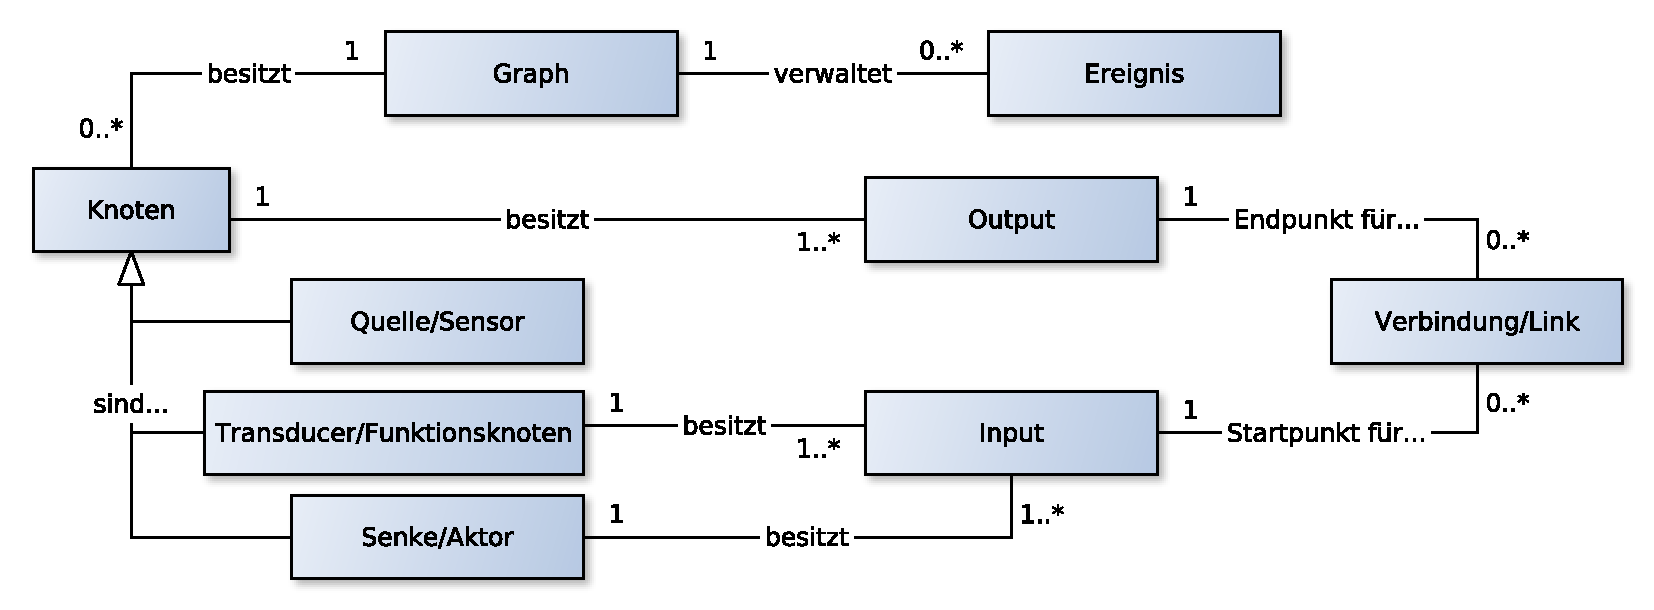
\includegraphics[width=0.95\textwidth]{bilder/chapter4/chapter4_2/domainmodelldatenfluss2.pdf}
  \caption{Das Domänenmodell des eines Datenflussprogrammes (in flowws) besteht aus drei Sorten von Knoten: Quellen/Sensoren, Senken/Aktoren und Funktionsblöcke/Transducer. Sie besitzen (mit Ausnahme der Quelle) Output- und Input-Interfaces, die es den Knoten erlauben durch Verbindungen/Links zu kommunizieren}
  \label{fig:bfddomainmodel}
\end{figure}
\begin{itemize}
    \item \textbf{Quellen} erzeugen die zu verarbeitenden Daten. Innerhalb von flowws bzw. cBlocks Netzwerken werden (virtuelle) Konstanten und (physische) Sensoren als datenerzeugendende Quellen angesehen. 
    \item \textbf{Funktionsknoten/Transducer} verarbeitenden Daten. Jeder Funktionsblock ist eine \textit{Black Box}, die aus einer Anzahl von Input-/Output-Schnittstellen und einer Verarbeitungslogik bestehen. Die Verarbeitungslogik wird im Falle von flowws von den funktionellen Anforderungen FA\#1 bis FA\#6 (Kapitel \ref{subsec:fanf}) vorgegeben. Nicht nur die Transformationen von Daten sondern auch temporale Operationen wie die zeitliche Verzögerung eines Signals werden in diesen Knoten abgearbeitet. 
    \item \textbf{Senken} konsumieren die erzeugten/verarbeitenden Daten. Innerhalb von flowws bzw. cBlocks Netzwerken übernehmen (virtuelle) Schnittstellen zu (physischen) Aktoren diese Aufgabe. Sie verwenden die erzeugten Daten, um ein bestimmtes Verhalten in Aktoren innerhalb des Systems herbeizuführen.
    \item \textbf{Verbindungen} transferieren Signale bzw. Nachrichten zwischen den Knotenpunkten. Sie definieren die eins-zu-eins Verbindung zwischen den Input/Output-Schnittstellen der Funktionsblöcke. Diese Verbindung ist gerichtet d.h. Daten fließen immer nur in eine Richtung durch den Graphen.
    \item \textbf{Ereignisse} sind Nachrichten, die durchd en Graphen von Node zu Node fließen. Sie beinhalten neben einem \textit{Payload}, der die eigentlichen Daten besitzt, auf dem die Transformationen durchgeführt werden, noch zusätzliche Metainformationen, die für die Bearbeitung der Daten wichtig sind. Die Datentypen, die der \textit{Payload} in besitzen kann wird von cBlocks-Ökosystem festgelegt und kann in Tabelle \ref{tab:datentypenpayloads} nachgeschlagen werden.
\end{itemize}

 \begin{table}[h]
\caption{Die drei verschiedenen Datentypen von Ereignis-\textit{Payloads}, die innerhalb von flowws verwendet werden.}
\label{tab:datentypenpayloads}
\begin{tabularx}{\textwidth}{llXX}
\hline
\rowcolor[HTML]{EFEFEF} 
Datentyp & Beispiel &  Erläuterung &  Verwendung \\ \hline
Number & 0,1,2,3.43,-12...& nummerischer Wert (Ganzzahlig und Fließkomma) & Temperatur, Abstand, Helligkeit, ...   \\ \hline
String & "qwnTZ32" & beliebige Zeichenkette & RFID-Code, Farbcodes, Display-Text, ... \\ \hline
Boolean & true, false & Wahrheitswert & Taster, Relays, ... \\ \hline
\end{tabularx}
\end{table}

\ac{DBP} erlaubt es effizient die Komplexität von parallelen \textit{Events} zu modellieren und auch für nicht Experten zu visualisieren. Dies ist somit ein guter Ansatz um die Anforderungen \hyperref[tab:NFA2]{NFA\#2} und \hyperref[tab:NFA0]{NFA\#0} zu bewältigen. Um \hyperref[tab:NFA0]{NFA\#0} allerdings komplett zu erfüllen, muss ein weiterer Sachverhalt adressiert werden: das modellieren sequentieller Logik, wie sie in Problem ''Parallel contra Sequentiell'' beschrieben und in  \hyperref[szenario2]{Szenario \#2} verdeutlicht ist.
\subsection{State-Machine-basierte Programmierung}\label{subsec:fsmprogrammierung}
\begin{quote}
    ''\textit{Have you tried turning it off and on again?}''  \\ -- Ein Jeder, der die Macht von \acp{FSM} verstanden hat.
\end{quote}

Bis zum jetzigen Zeitpunkt kann man den beschriebenen \ac{DBP}-Ansatz mit dem von SAM Labs (Kapitel \ref{subsubsec:samlabs}) vergleichen, auch mit seinen Problem (''Sequentiell contra Parallel'' und ''Signalpriorisierung''). Wie schon in den Problemen beschrieben, muss es Aktoren möglich sein mit parallel eintreffenden Signalen umgehen zu können, um Szenarien wie die in \hyperref[szenario2]{Szenario S\#2}  beschriebene Ampelschaltung und die in \hyperref[szenario3]{Szenario S\#3} beschriebene Vermeidung von Signalkonflikten zu ermöglichen.

Die einzige Möglichkeit für SAM Labs diesen Problemen aus dem Weg zu gehen ist es, sequentielle Logik mit der Datenfluss-Logik zu vermischen. Dies geschieht indem die Steuerungslogik der Aktoren, welche Entscheidungen über das Verhalten des Aktors treffen, auf der selben Ebene deklariert werden, wie die Logik, die Signale in eine nutzbare Form transformieren. In flowws wird einen anderen Weg gegangen. Es kommt eine Paradigma zum Steuern der Aktoren, welches weite Verbreitung in der IT und in \textit{Embedded Hardware} genießt: die \acl{FSM} (dt. ''endlicher Zustandsautomat'')

\begin{figure}[h]
  \centering
  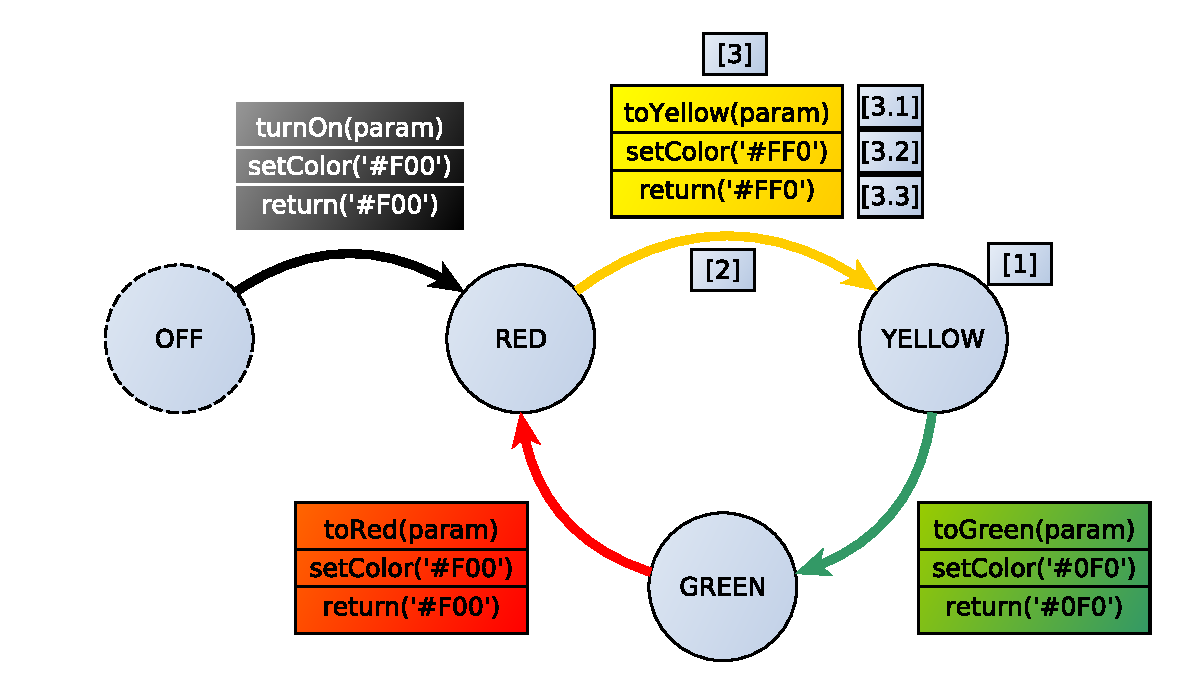
\includegraphics[width=0.85\textwidth]{bilder/chapter4/chapter4_2/beispielstatemachine.pdf}
  \caption{Die \ac{FSM} eines cBlocks mit LED-Aktor. Es existieren vier Zustände: OFF (Startzustand), RED, YELLOW, GREEN; und vier Übergänge: turnOn(), toYellow(), toGreen() und toRed(). Jeder der Übergänge verwendet in diesem Fall die setColor()-Funktion des LED-Aktors um die LED in der jeweils definierten Farbe wechseln. Jeder Übergang nimmt die Parameter (param) entgegen, was dem \textit{Payload} eines \textit{Events} entspricht. Dieser wird in diesem Beispiel entgegen genommen aber nicht verwendet. Zusätzlich erzeugt jeder Übergang mit return(<farbcode>) ein weiteres Event.}
  \label{fig:beispielfsm}
\end{figure}

\acp{FSM} sind Systeme von einer endlichen Menge von Zuständen (engl. ''States''), die auf eine endliche Menge von Ereignissen (engl. ''Events'') reagieren, welche außerhalb des Systems auftreten und auf das System einwirken. Die Reaktion einer \ac{FSM} auf eintreffende Signale werden abhängig einer endlichen Anzahl von Übergängen (engl. ''Transitions'') gesteuert. Wenn eine \ac{FSM} zu jeder Zeit nur einen Zustand annehmen kann, ist sie \textit{deterministisch} (\cite{hopcroft2013introduction}). 

Die Parallelen zu cBlocks bzw. flowws werden hierbei klar: cBlocks-Aktoren können als \acp{FSM} dargestellt werden. Ein Beispiel ist in Abbildung \ref{fig:beispielfsm} in Form eines LED-cBlocks gegeben, der eine Ampelschaltung modelliert. Es sind hierbei vier Elemente sichtbar, welche im Domänen-Modell (Abbildung \ref{fig:domainmodelfsm}) korrespondieren:
\begin{itemize}
    \item \textbf{Zustände/States [1]:} Ein Zustand drückt wie im \ac{FSM}-Modell den momentanen Status eines Automaten bzw. des Aktor-cBlocks aus. Diese Status ist nicht an die Ausprägung eines bestimmten Eigenschaft des Aktors gebunden, sprich ''RED'' bedeutet nicht zwangsweise die Farbe Rot. Vielmehr legt ein Zustand fest, welche zukünftigen Zustände beim eintreffen des nächsten Ereignisses erreichbar sind. In Abbildung \ref{fig:beispielfsm} ist es bspw. nicht möglich von Status ''RED'' in ''GREEN'' direkt zu springen. Durch dieses Konstrukt, lässt sich sequentielles Verhalten in den cBlock einprogrammieren. Zusätzlich existiert ein Anfangszustand, der die initiale Ausprägungen des cBlock-Aktors definiert.
    \item \textbf{Übergänge/Transitions [2]:} Die Übergänge werden ebenfalls durch den Nutzer definiert. Sie verbinden die einzelnen Zustände und modellieren das Verhalten eines cBlocks. Übergänge gestatten/verbieten durch ihre Existenz/Abwesenheit eine Signalpriorisierung vorzunehmen. Eine \ac{FSM} erlaubt es die Logik des cBlocks graphisch so zu modellieren, dass ein (zum momentanen Status) im Konflikt stehendes eintreffendes Signal ignoriert wird.
    \item \textbf{Übergangslogik/Transitional Logic [3]:} Die Logik, welche die Eigenschaften (Tabelle
\ref{tab:typesOfActutors}) eines Aktor-cBlocks manipuliert und somit physikalische Signale erzeugt, ist innerhalb der Übergänge. Sie besteht im Grunde aus drei Teilen:
    \begin{itemize}
        \item Die \textbf{Deklaration [3.1]} gibt den Namen des Übergangs an, der nach außen hin als Input-Schnittstelle sichtbar ist. Der Parameter der Deklaration symbolisiert den Payload, des eintreffenden Ereignisses und kann optional von der Funktionslogik weiterverarbeitet werden.
        \item Die \textbf{Funktionslogik [3.2]} beinhaltet die konkreten Instruktionen, die die Eigenschaften des cBlocks manipulieren. In Abbildung \ref{fig:beispielfsm} wird bspw. \texttt{setColor(<farbe>)} verwendet um die Farbe der LED zu ändern. Diese Funktionen sind für jeden Aktor speziell und werden von den cBlocks selbst vorgegeben. Experten (z.B. Persona ''Mark'') können allerdings weitere Funktionen hinzufügen und somit den Funktionsumfang eines Aktors für Laura erweitern.
        \item Der \textbf{Rückgabewert [3.3]} gibt ähnlich wie die Deklaration, eine Schnittstelle der Aktor-\textit{Black Box} an. In diesem Fall allerdings eine Output-Schnittstelle. Durch diese Schnittstellen kann ein Aktor seine Zustandsänderung, in Form eines neuen Ereignisses, dem Rest des Systems mitteilen. 
    \end{itemize}
\end{itemize}

\begin{figure}[h]
  \centering
  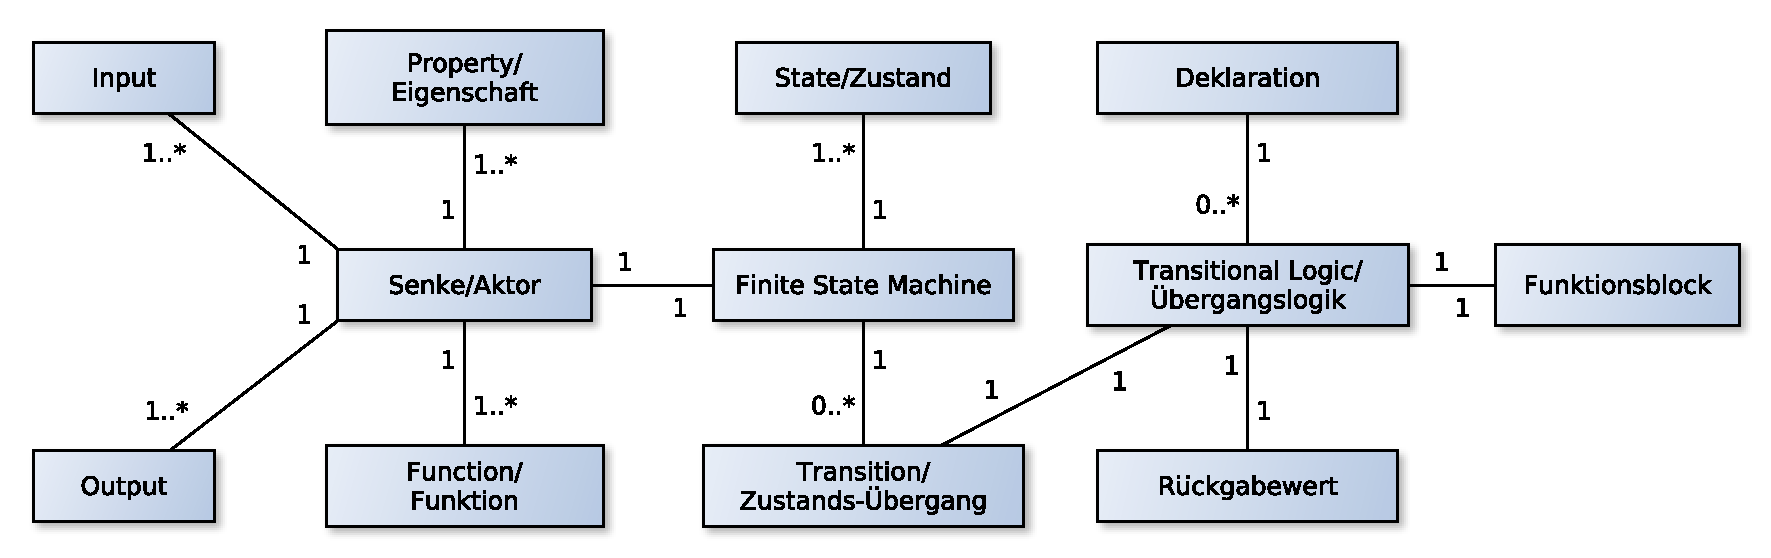
\includegraphics[width=1\textwidth]{bilder/chapter4/chapter4_2/domainmodellaktor.pdf}
  \caption{Das Domänenmodell des Aktors bzw. der \ac{FSM} ist eine Detailansicht von Abbildung \ref{fig:bfddomainmodel} hinsichtlich der Bestandteile des Aktors. }
  \label{fig:domainmodelfsm}
\end{figure} \hyperref[]{}

Durch das Verwenden einer \ac{FSM} ergeben sich mehrere Vorteile. Durch die gute Visualisierung der \ac{FSM} und der weiten Verbreitung des Modells kann die Erlernbarkeit gefördert und somit \hyperref[tab:NFA2]{NFA\#2}, adressiert werden. Zusätzlich erlaubt das Benutzen von \ac{FSM}, wie in  \hyperref[tab:NFA0]{NFA\#0} gefordert, sequentielles Verhalten zu modellieren, indem es die asynchronen Ereignisse, die auf den Aktor-cBlock einwirken, sequentiell zu verarbeiten. Das Hinzufügen von zusätzlichen Aktor-Funktionen durch Experten, kann das System nachträglich erweitert werden, wie es von  \hyperref[tab:NFA5]{NFA\#5} verlangt ist. Im nächsten Schritt muss geklärt werden, wie \ac{DBP} und \ac{FSM} miteinander integriert werden, um Endnutzern das Entwickeln von Programmen innerhalb von flowws zu ermöglichen.
\subsection{flowws}
In den zwei vorangegangenen Kapiteln wurden die zwei Paradigmen beschrieben, welche die Anforderungen bezüglich des Programmiermodells erfüllen sollen, namentlich die sequentielle und parallele Programmierung der cBlocks in visueller Form. Im Folgenden, wird das Zusammenspiel beider Paradigmen erklärt. Dabei wird auf das Konzeptmodell, Ausführungsmodell und die Eigenheiten von flowws bezüglich des cBlocks-Kontext eingegangen. Dieses Modell und die visuelle Darstellung sind die zentralen Bestandteile von flowws.

\begin{figure}[h]
  \centering
  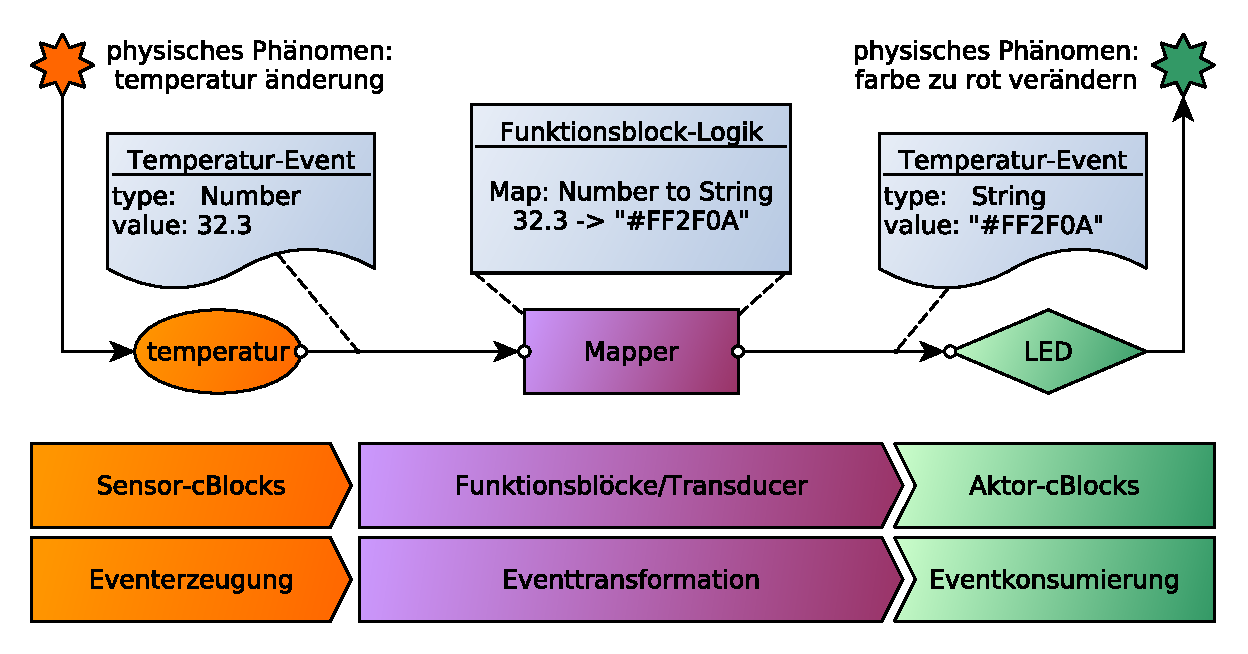
\includegraphics[width=1\textwidth]{bilder/chapter4/chapter4_2/flowwsschematicexample.pdf}
  \caption{Ein schematisches Beispiel für das Ausführungsmodell von flowws. Die Daten fließen von der Erzeugung als Events durch Funktionsknoten um zu transformiert zu werden. Dadurch erhalten sie einen höheren semantischen Wert, sodass sie vom Aktor konsumiert werden können.}
  \label{fig:beispielflowws}
\end{figure}

In Abbildung \ref{fig:beispielflowws} wird ein in flowws modelliertes Programm bzw. Graph schematisch dargestellt.  In diesem Beispiel, wird von einem Temperatur-Sensor ein Temperatur-Event erzeugt, welches die Farbe der LED manipulieren soll (blau für kalt, rot für warm). Hierbei wird ein Funktionsknoten verwendet, der den \texttt{Number}-Wert des Events auf eine Wertebereich von Farben abbildet. Dieses semantisch höherwertige Event wird dann vom Aktor bzw. der \ac{FSM} des Aktors verwendet, um dessen Zustand zu ändern. Hierbei wird das Kernprinzip von flowws, das sich in in drei Schritte aufteilt, verdeutlicht:

\subsubsection{1. Eventerzeugung}
 Eventerzeugung ist die erste Phase jedes flowws-Programmes. Jeder Sensor-cBlock, der mit dem System verbunden ist, besitzt einen virtuellen Sensorknoten als Repräsentant. Jeder Sensorknoten entspricht einem cBlock, d.h. cBlocks die mehrere unterschiedliche Events erzeugen (bspw. ein cBlock der Temperatur und Luftfeuchtigkeit misst) werden als einen Knoten mit mehreren Ausgängen dargestellt. 
 
 Wie in Abbildung \ref{fig:seqsensorblock} gezeigt, erzeugen Sensorknotens kontinuierlich Ereignisse mit Rohdaten als \textit{Payload}, auf Basis physikalischer Phänomene (z.B. Temperaturschwankungen). Diese Rohdaten haben oftmals keine semantische Bedeutung und sind in vielen Fällen schlichtweg Zahlenwerte oder Zeichenketten (siehe Tabelle \ref{tab:datentypenpayloads}).
 
 \begin{figure}[h]
  \centering
  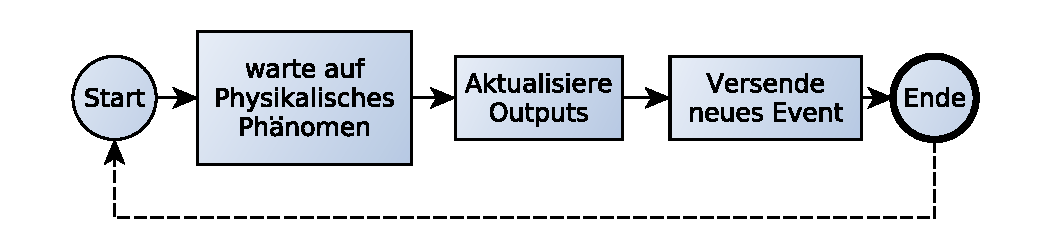
\includegraphics[width=1\textwidth]{bilder/chapter4/chapter4_2/sensorblockablauf.pdf}
  \caption{Standardablauf innerhalb eines Sensorknotens, wenn ein physikalisches Ereignis erfolgt ist.}
  \label{fig:seqsensorblock}
\end{figure}

 Wie alle anderen Knoten innerhalb von flowws sind auch Sensorknoten \textit{Black Boxen}. Der Unterschied zu anderen Knoten ist allerdings, dass sie keine Eingänge besitzen, sondern ausschließlich Ausgänge als Schnittstellen, da sie selbst nicht in ihrem Verhalten beeinflusst werden sollen. Dies soll die Verbindung zum physikalischen Sensor cBlock stärken, da es intuitiv ist, dass Aktoren ein aktives Verhalten besitzen während Sensoren passiv ihre Umgebung wahrnehmen. 
 
 \subsubsection{2. Eventtransformation}\label{subsubsec:eventtrans}
 Bei der Eventtransformation kommt dass \ac{DBP}-Paradigma aus Kapitel \ref{subsection:datenflussprog} zu tragen. Die erzeugten Daten werden durch eine Reihe von Funktionsknoten geleitet und somit miteinander kombiniert und/oder transformiert. 
 
 Der Ablauf einer Transformation innerhalb eines Funktionsknotens ist in Abbildung \ref{fig:seqfunktionsblock} dargestellt.
 \begin{figure}[h]
  \centering
  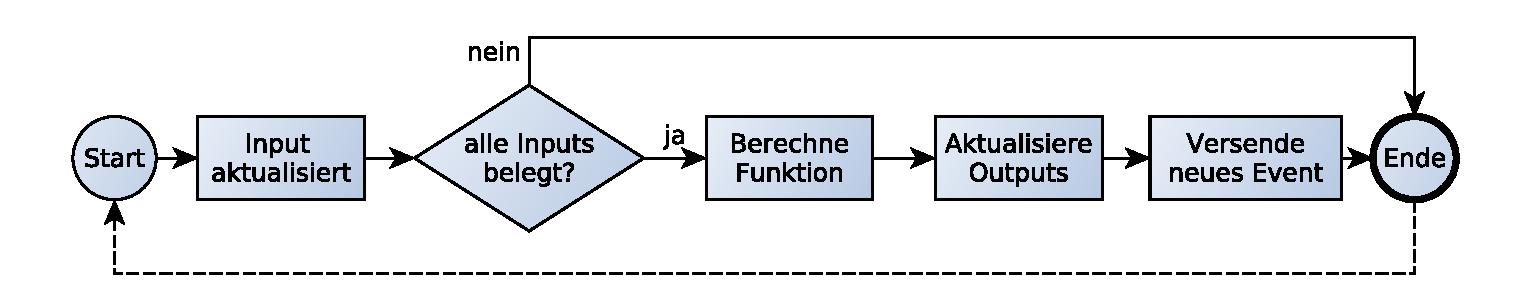
\includegraphics[width=1\textwidth]{bilder/chapter4/chapter4_2/funktionsblockablauf.pdf}
  \caption{Standardablauf innerhalb eines Funktionsknotens, wenn eine Input-Schnittstelle aktualisiert wird.}
  \label{fig:seqfunktionsblock}
\end{figure}
Wenn sich eine Input-Schnittstelle durch ein eintreffendes Ereignis aktualisiert wird, prüft der Transducer nach, ob sämtliche Input-Schnittstellen einen Wert besitzen. Der Knoten nimmt dann seine Transformation der Events vor, gibt das Ergebnis an die Output-Schnittstellen weiter, welche das neue Ereignis versenden. Folgendes ist hierbei zu beachten: 
\begin{itemize}
    \item Eingehende Signale werden nicht wie bei \ac{DBP} üblich, in der Input-Schnittstelle in einer \textit{Queue} gepuffert und nacheinander abgearbeitet, sondern überschrieben. Der Grund hierbei ist, dass cBlocks zu jeder Zeit auf den momentanen Zustand ihrer Umgebung reflektieren sollen. Es macht beispielsweise wenig Sinn, nicht mehr aktuelle Umgebungstemperaturen nacheinander abzuarbeiten.
    \item Events werden von Funktionsknoten nicht konsumiert. Aufgrund gleicher Überlegungen wie beim vorherigen Punkt, sollen die Events immer den momentanen Zustand der physischen Umgebung widerspiegeln, in der sich die (physischen) cBlocks befinden. Gibt es bspw. mehrere Sensoren mit unterschiedlichen Abtastfrequenzen müssen sämtliche Signale immer auf das Signal des Langsamsten warten. In solchen Fällen, wird das letzte Signal als das Aktuellste betrachtet und zur Durchführung der Funktion verwendet.
\end{itemize}
 Die Funktionen zur Transformation von Ereignissen, orientieren sich an den funktionalen Anforderungen \hyperref[tab:fanf]{FA\#1}  bis  \hyperref[tab:fanf]{FA\#6}:
 \begin{itemize} 
     \item Bei \textbf{Bool'schen Gattern} handelt es sich um logische Operationen, die auf ein oder mehrere bool'sche Signale angewandt werden. Zu den Funktionen zählen: Negation, logisches Und/Oder und exklusives Oder ($\neg, \land, \lor, \oplus$). Sie überprüfen den Ausdruck abhängig der Eingänge auf Wahrheit und geben das bool'sche Ergebnis weiter.
     \item Zu \textbf{Vergleichsoperationen} gehören sämtliche Operationen, die zwei Zahlen miteinander vergleichen können, und einen bool'schen Wert ausgeben ($<,\leq,=,\neq,\geq,>$).
     \item \textbf{Zeitgesteuerte Operationen} erlauben es dem Nutzer Signale auf ihre temporären Eigenschaften zu manipulieren d.h. Signale zeitlich zu verzögern oder Signale periodisch zu wiederholen.
     \item \textbf{Konvertierungsoperationen} wandeln Signale um, indem sie den Wertebereich des Eingangssignals auf einen vordefinierten Zielbereich des Ausgangssignals zuweisen. Dies kann auf zwei weisen geschehen: kontinuierliche Wertebereiche ($\left [ 1,2,3,...,n \right ] \rightarrow \left [ -n,...,-3,-2,-1 \right ]$) oder kategorische Wertebereiche ($\left [ \geq20, \leq30  \right ] \rightarrow \left [ kalt,heiss \right ]$)
     \item Der \textbf{Generische Operator} erlaubt es Experten ihre eigenen Transformationen in Programmcode zu beschreiben. Dieser Programmcode kann beliebig viele Ein- und Ausgänge besitzen sowie ein beliebige Kombination von Datentypen, solange sie mit denen von Tabelle \ref{tab:datentypenpayloads} übereinstimmen
 \end{itemize}
 Es können noch weitere vorgefertigte Funktionen definiert werden, allerdings würde dies den Rahmen dieser Arbeit hinausgehen und wäre nicht Zielführend, führ die Definition eines \ac{EUD}-Systems. Allerdings wird durch Funktionsknoten mit Nutzer-definierter Logik eine Schnittstelle vorgesehen, die es dem Endnutzer erlaubt, eigene Transformationslogik einzuprogrammieren. Somit wird dem Endnutzer erlaubt, flowws durch jede beliebige Funktion zu erweitern.
 
\subsubsection{3. Eventkonsumierung} \label{subsubsec:evebtkonsumierung}
Mit dem Konsumieren der Events schließt sich der Kreis, indem ein initiales physisches Phänomen, dass durch die Sensor-cBlocks aufgenommen wurde in einem neuen physischen Phänomen, dass vom Aktor-cBlock erzeugt wird (siehe Abbildung \ref{fig:beispielflowws}). 

Jeder Aktor-cBlock, der mit flowws verbunden wird, ist ähnlich wie bei den Sensor-cBlocks mit einer virtuellen Abbild (hier: Aktorknoten) repräsentiert. Ein Aktorknoten ist intern eine \ac{FSM} wie sie in Kapitel \ref{subsec:fsmprogrammierung} beschrieben. Hierbei werden vom Endnutzer Zustände, Übergänge und Übergangslogik definiert um dem Aktor ein gewünschtes Verhalten zu geben.

 \begin{figure}[h]
  \centering
  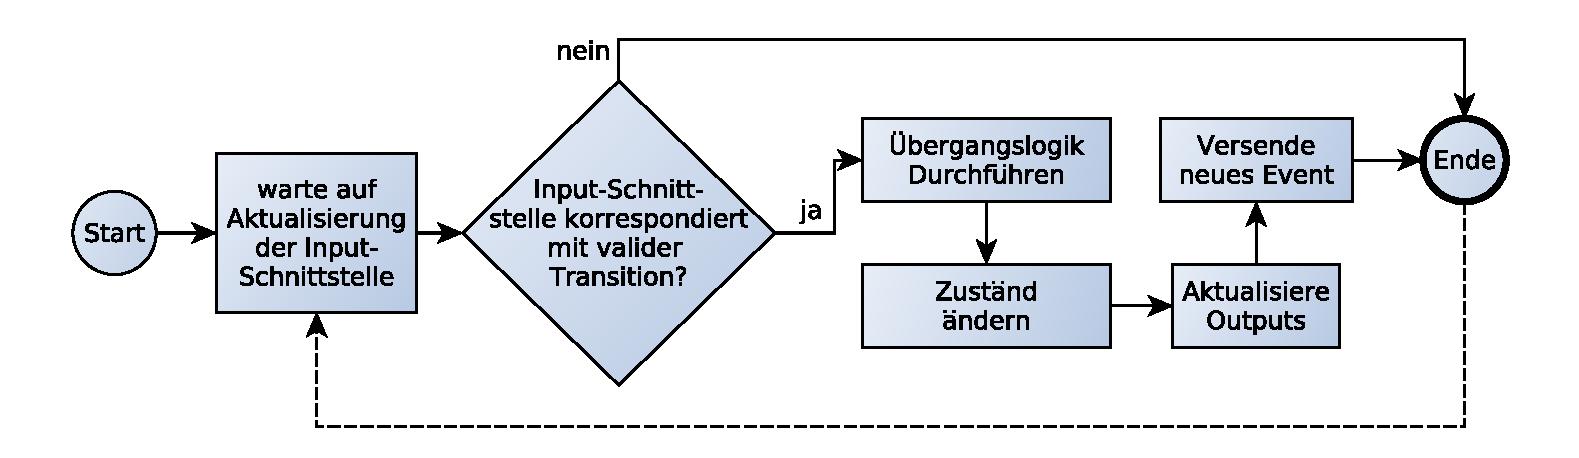
\includegraphics[width=1\textwidth]{bilder/chapter4/chapter4_2/aktorblockablauf.pdf}
  \caption{Standardablauf innerhalb eines Aktorknotens, wenn eine Input-Schnittstelle aktualisiert wird.}
  \label{fig:seqaktorblock}
\end{figure}

Jeder Aktorknoten besitzt zusätzlich zu seiner \ac{FSM} zwei weitere Komponenten:
\begin{itemize}
    \item \textbf{Aktoreigenschaften} sind alle Eigenschaften, welche die Art des physikalische Signals beeinflussen. Ein LED-cBlock kann die Aktoreneigenschaften \texttt{(r,g,b)} und \texttt{(Brightness)} besitzen; ein Lautsprecher-cBlock kann die Eigenschaften \texttt{(AudioFrequency)} und \texttt{(Volume)} besitzen oder ein LCD-cBlock kann die Eigenschaft \texttt{(DisplayText)} besitzen. Vorgegeben werden diese Eigenschaften von dem cBlocks \textit{Back-end}. Auf Hardwareebene werden solche Aktoreneigenschaften als \textbf{Ressource} bezeichnet. Von diesem abstrakten Begriff wird aufgrund von Benutzerfreundlichkeit allerdings in flowws Abstand genommen.
    \item \textbf{Aktorfunktionen} sind der einzige Weg innerhalb von flowws, Aktoreigenschaften direkt zu manipulieren. Jeder Aktorknoten wird mit einem Menge von Funktionen geliefert. Diese bestehen aus Funktionen wie \texttt{setColor()}, \texttt{setBrightness()}, \texttt{setFrequency()}, etc; und ermöglichen dem Endnutzer den Aktor durch geschickte Modellierung der Übergangslogik zu manipulieren. Anders als die Aktoreigenschaften besitzen Experten die Möglichkeit, zusätzliche Funktionen hinzufügen und somit die Flexibilität von Aktoren bei der Manipulation ihrer Eigenschaften erhöhen.
\end{itemize}

In Abbildung \ref{fig:seqaktorblock} ist der Ablauf zu sehen, der Durchgeführt wird, sobald ein neues Ereignis eintrifft. Zuerst ermittelt der Aktorknoten mit welchem Übergang die aktualisierte Input-Schnittstelle korrespondiert. Als Nächstes wird überprüft ob der Übergang erlaubt ist abhängig von dem Zustand, indem sich der Aktorknoten momentan befindet. Ist dies der Fall, wird die Übergangslogik ausgeführt und abhängig davon, des Events und der Aktorfunktionen die Eigenschaften des Aktors verändert. Durch die Veränderung der Aktoreigenschaften wird ein physikalisches Signal erzeugt. Ebenso kann ein neues Signal erzeugt werden und über eine Output-Schnittsstelle, welches ebenfalls mit der Übergangslogik korrespondiert, versendet werden. Ein Aktorknoten ist somit mehr als nur ein Konsument; er kann wie ein Sensorknoten neue Signale erzeugen, welche wiederum transformiert und von weiteren Aktorknotens konsumiert werden können.

\subsubsection{Zusammenfassung}
Hiermit wurde das Programmiermodell von flowws geklärt, eine Fusion von \ac{DBP} und \ac{FSM}. Es handelt sich hierbei um eine neues Programmiermodell, welches noch nicht innerhalb eines \ac{EUD}-Werkzeugs verwendet wurde. Aus diesem Grund, kann noch keine objektive Aussage über die Effektivität des Modells hinsichtlich Benutzerfreundlichkeit gemacht werden. Nichtsdestotrotz kann man die erhofften Vorteile logisch schlussfolgern:
\begin{itemize}
    \item \textbf{zu \hyperref[tab:NFA0]{NFA\#0} -- Sequentielle und Parallele Programmierung} Das Problem aus Kapitel \ref{sec:problemanalyse} wurde durch die Kombination von \ac{DBP} und \ac{FSM} beseitigt.
    \item \textbf{zu \hyperref[tab:NFA2]{NFA\#2} -- Leicht Erlernbar} Das Modell basiert auf \ac{DBP} und \ac{FSM}. Beides sind Konzepte die in der Informatik und Elektrotechnik weite Verbreitung finden. Diese Beliebtheit haben beide Konzepte ihrer Fähigkeit schwere Konzepte (Parallelität und \textit{State-Management}) intuitiv darzustellen zu verdanken. Zusätzlich sind Konzepte wie \ac{DBP} und \ac{FSM} auch in verschiedenen Werkzeugen die häufig von Designern verwendet werden (bspw. \textit{Game Engines} und 3d Modellierungs Software). Es besteht also eine gute Chance, dass auch nicht Experten die Konzepte von flowws schnell erlernen können.
    \item \textbf{zu \hyperref[tab:NFA2]{NFA\#2} -- Leichter Verständlich} \ac{DBP} und \ac{FSM} besitzten Pendants in der UML. Aus diesem Grund, lassen sich beide Teile gut graphisch Darstellen. Die bildliche Darstellung sollte eine bessere Verständlichkeit über die Vorgänge innerhalb des Programmes führen und somit etwaige Fehlersuche beschleunigen.
    \item \textbf{zu \hyperref[tab:NFA5]{NFA\#5} -- Flexibel} flowws bringt mit Funktionsknoten und Aktorfunktionen viel vorgefertigte Programmlogik mit. Allerdings können beide Elemente auch durch Experten erweitert werden um flowws optimal auf den Anwendungsfall anzupassen.
   
\end{itemize}

Im nächsten schritt wird die graphische Oberfläche und Darstellung der einzelnen Elemente sowie die Interaktionen mit ihnen geklärt.
\section{Graphisches Modell}\label{sec:graphischesmodell}
Im vorherigen Kapitel wurde das grundlegende Programmierungskonzept von flowws erklärt und anhand der Anforderungen gegenüber dem System sowie anhand der Probleme bestehender Systeme begründet. Wie allerdings schon in der Einleitung (Kapitel \ref{sec:einleitungkonzept}) geschrieben, benötigt die \ac{EUD} eine graphische Oberfläche, mit welcher der Endnutzer interagieren kann. Entscheidungen anhand von Anforderungen, Probleme und \ac{CD} rationalisiert.
 
\subsection{Design Richtlinien}
Für die graphische Oberfläche von flowws müssen die einzelnen Elemente, die im vorherigen Kapitel beschrieben wurden, durch eine graphischen Repräsentant abgebildet werden. Der Endnutzer muss mit diesen Abbildungen interagieren, um die gewünschte Betriebsverhalten des Gesamtsystems zu erreichen. Um eine kohärente \ac{UX} zu erreichen, sollen Abbildung und Interaktion einer geteilten Philosophie unterliegen; einem Satz von Regeln, der die Design-Entscheidungen rationalisiert und sich an den Rahmenbedingungen des Projekts orientiert.

\paragraph{Nähe zur Realität}\label{par:naehezurrealitaet} Es sollte immer bedacht werden, dass die (physischen) cBlocks zu jedem Zeitpunkt des Design Prozesses verwendet werden. Graphisch soll diese physische Bindung reflektiert werden. Aus diesem Grund soll die visuelle Darstellung und die Interaktionen der \ac{EUD} wenn möglich Bezug zu den cBlocks oder zumindest mit der Domäne der \ac{IoT} und Elektrotechnik besitzen. Es wird sich dadurch erhofft, dass \textbf{Domänennähe} und \textbf{funktionale Aussagekraft} (siehe Tabelle \ref{tab:cognitivedimensions}) zu erhöhen und somit die Anforderungen \hyperref[tab:NFA2]{NFA\#2} und  \hyperref[tab:NFA3]{NFA\#3} zu lösen.

\paragraph{Fokus bewahren}\label{par:fokusbewahren} Design ist ein kreativer Prozess von dem flowws nicht durch seine eigene Komplexität ablenken soll. Um schnell und zielführend Arbeiten zu können, soll flowws Vorgaben machen an denen sich der Endnutzer orientieren kann. Durch graphische Signale wie Farben und Formen, soll dem Nutzer das Rätseln über die Rolle einzelner Komponenten erspart werden.

\paragraph{Fehler vorbeugen}\label{par:fehlervorbeugen} Statt zeitaufwändige Fehlersuche zu unterstützen ist es sinnvoller, Fehler durch graphische Hinweise im Vorfeld zu vermeiden (siehe Tabelle \ref{tab:cognitivedimensions} und  \hyperref[tab:NFA4]{NFA\#4}).

\paragraph{'\textit{'Move fast and break things}''}\label{par:movefast} Prototyping ist schnell und explorativ. Deswegen soll die \ac{GUI} von flowws diese schnelle Art von Arbeit durch bspw. Austauschbarkeit der Komponenten unterstützen.

\paragraph{''\textit{Grow-As-You-Go}''}\label{par:growasyougo} flowws ist kein Lehrwerkzeug sondern soll produktives Arbeiten ermöglichen. Die technischen Fähigkeiten der Endnutzer sind allerdings sehr Variabel. Zusätzlich ist zu erwarten, dass das technische Verständnis mit der stetigen Benutzung des Werkzeugs wächst. Daher soll der Funktionsumfang der Oberfläche mit den Fähigkeiten des Endnutzers wachsen können. Das Erlernen der Oberfläche durch nützliche Hinweise unterstützen (siehe \hyperref[tab:NFA2]{NFA\#2}). Gleichzeitig aber soll sie nicht obsolet werden, bei komplexeren Szenarien, in denen spezifischere Funktionalität abverlangt wird (siehe  \hyperref[tab:NFA5]{NFA\#5}).

%%%%%%%%%%%%%%%%%%%%%%%%%%%%%%%%%%%%%%%%%%%%%%%%%%%%%%%%%%%%%%%%%%%%%%%%

\subsection{Workspace}
\begin{figure}[h]
  \centering
  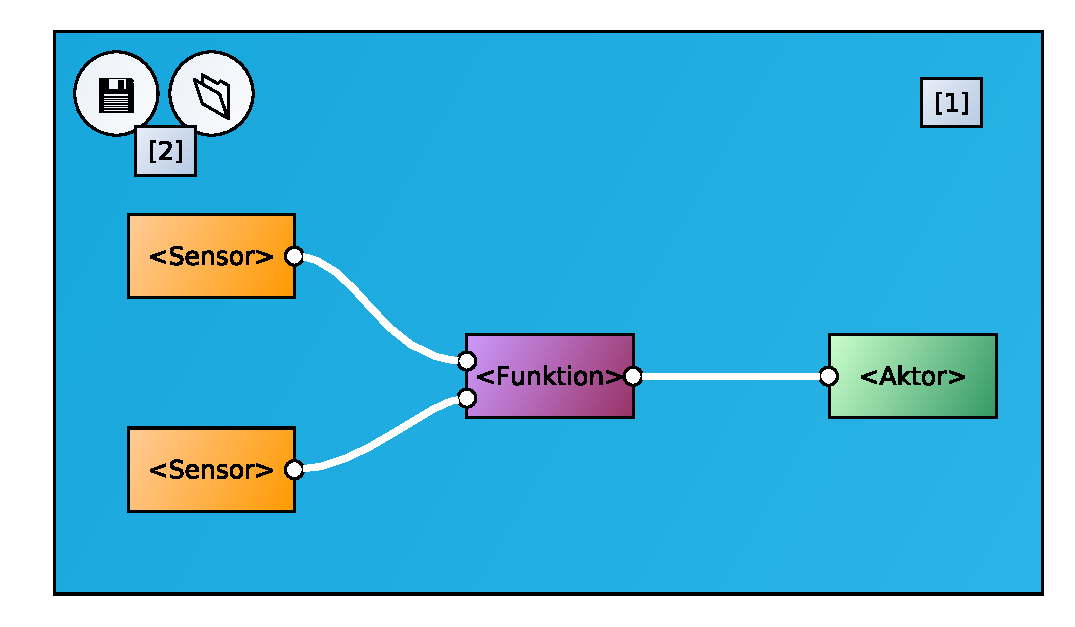
\includegraphics[width=.75\textwidth]{bilder/chapter4/chapter4_3/workspace.pdf}
  \caption{[1] ist der Workspace mit einem generischen Graph. [2] sind Funktionen, die es erlauben die Graphen zu verwalten.}
  \label{fig:workspace}
\end{figure}


\paragraph{Kurzbeschreibung} Der Workspace (dt. ''Arbeitsbereich'') ist die primäre Komponente von flowws. Innerhalb dieser Komponente werden flowws-Graphen bzw. flowws-Programme erstellt, organisiert, administriert und auf Fehler untersucht. Er dient als digitale Leinwand für den Designer, um im Zusammenspiel mit den physischen cBlocks Prototypen zu erstellen.

\paragraph{Rahmenbedingungen \& Entscheidungen} Der digitale Arbeitsbereich, soll den physischen Arbeitsbereich nachbilden. flowws wird immer simultan zu cBlocks verwendet, d.h. der Endnutzer manipuliert und interagiert während des gesamten Entwicklungszyklus mit den cBlocks. Aus diesem Grund, arbeitet der Endnutzer zu jederzeit an maximal einem Graphen. Dies steht im Kontrast zur Programmierung in \acp{IDE}, in denen an mehreren Projekten simultan gearbeitet werden kann und somit ein hoher Grad von Kontextwechsel benötigt wird. Bei flowws soll sich der Designer ähnlich wie bei einer Leinwand vollständig auf die Erstellung des Graphen konzentrieren können, ohne sich mit einer Kakophonie von Icons und Untermenüs auseinandersetzen zu müssen. 

\textbf{Aktionen}, die von und in dieser Komponente durchgeführt werden können: 
\begin{itemize}
    \item \textbf{Anzeigen von Knoten} Der Workspace dient dem Anzeigen von Sensor-, Aktor- und Funktionsknoten. 
    \item \textbf{Administration von Graphen} Der Graph kann über den Workspace gespeichert, geladen und verwaltet werden. 
\end{itemize}

\paragraph{Darstellung} Der Workspace bewusst schlicht gehalten, wie in Abbildung \ref{fig:workspace} gezeigt wird. Bis auf zwei Knöpfe zum Laden und Speichern von Graphen sind keine weiteren Interaktionsmöglichkeiten zu sehen. Diese Entscheidung wurde bewusst so getroffen. Der leere Workspace soll einen leeren Schreibtisch nachahmen (siehe ''Nähe zur Realität''). Aus diesem Grund, werden Sensorknoten und Aktorknoten automatisch angezeigt, wenn ihre physischen Gegenstücke mit dem System verbunden sind. Die Schreibtisch-Metapher soll unterstützt werden, indem die Optik des Workspace an eine typische Schneideunterlage, wie sie in Werkstätten zu finden ist, angelehnt.

%%%%%%%%%%%%%%%%%%%%%%%%%%%%%%%%%%%%%%%%%%%%%%%%%%%%%%%%%%%%%%%%%%%%%%%%

\subsection{flowws-Graph}
\subsubsection{Knoten}
\begin{figure}[h]
  \centering
  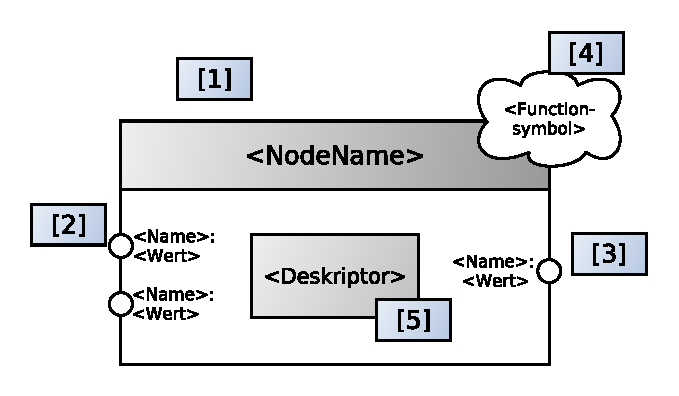
\includegraphics[width=.8\textwidth]{bilder/chapter4/chapter4_3/genericnode.pdf}
  \caption{Ein generischer Knoten.}
  \label{fig:genericnode}
\end{figure}

\paragraph{Kurzbeschreibung} Knoten sind die fundamentalen Bausteine eines jeden flowws-Graphen. Sie erzeugen, transformieren und konsumieren Daten auf die Weise, auf die sie vom Endnutzer kompositioniert und konfiguriert sind. Alle Knoten (Sensoren, Funktionen, Aktoren) teilen fundamentale Charakteristiken (Identität, Form), Subkomponenten (Input-/Output-Schnittstellen, Deskriptor) und Interaktionen (Anordnen, Erstellen, Löschen) miteinander. 

\paragraph{Rahmenbedingungen \& Entscheidungen} Jeder Block muss eindeutig von seinem Typus identifizierbar und seinem physischen Pendant zuordenbar sein. Da es viele Arten von Knoten gibt, muss es möglichst leicht erkenntlich sein, welche Funktion er übernimmt, welche Daten ein- und ausfließen und aus welchem Grund der Block seine Entscheidung getroffen hat.

\textbf{Aktionen}, die von und in dieser Komponente durchgeführt werden können: 
\begin{itemize}
    \item \textbf{Anordnen} Die Knoten lassen sich hinsichtlich ihrer Position organisieren bzw. anordnen. Dadurch kann der Endnutzer die Position der physischen Aktoren/Sensoren mit denen der Virtuellen abgleichen (siehe ''Nähe zur Realität'').
    \item \textbf{Verbindung starten/enden} Die Schnittstellen dienen als Interaktionspunkte um Verbindungen zu starten und zu enden.
    \item \textbf{Deskriptor ändern} Durch das ändern des Deskriptors kann das Verhalten von Knoten auf Eingangssignale konfiguriert werden.
\end{itemize}

\paragraph{Darstellung} Der in Abbildung \ref{fig:genericnode} dargestellte generische Block besitzt alle Merkmale, die in Aktor-,Sensor- und Funktionsknoten vorhanden sind. Die quadratische Darstellung des Knoten wurde einer komplexeren Darstellung bevorzugt, um eine visuelle Nähe zum Quader-Design der cBlocks zu erreichen (siehe Abbildung \ref{fig:cblockfoto}). \textbf{[1]} ist die Identifikationsleiste des Blocks. Sie gibt durch Farbe Aufschluss über den Typ (\colorbox{sensororange}{Sensor}, \colorbox{aktorgreen}{Aktor} und \colorbox{funcviolet}{Funktion}) und durch Text Aufschluss über die Rolle (z.B. ''Logisches-Gatter'') des Knotens. \textbf{[2]} und \textbf{[3]} sind die Input- und Output Schnittstellen. Sie dienen als Anfangs- und Endpunkte für Verbindungen, besitzen Namen durch die sie Unterscheidbar werden (''OperandA'' etc.) und zeigen den letzten Wert an, der über die Schnittstelle empfangen bzw. versendet wurde (siehe \hyperref[tab:NFA1]{NFA\#1}). \textbf{[4]} ist der Knoten-Indikator und gibt wie \textbf{[2]} Aufschluss über den Knotentyp und Knotenrolle. Er zeigt zum einen durch seine Form den Typ und zum Anderen mit einem Symbol die konkrete Rolle des Knotens (bspw. Sensorknoten: Temperatur, Funktionsknoten: Logisches-Gatter, etc.) an. \textbf{[5]} ist der Knoten-Deskriptor. Er gibt Endnutzer Aufschluss, welche konkrete Instruktion (bspw. logisches Und) auf den Eingabedaten ausgeführt werden bzw. in welchem Zustand sich der Knoten momentan befindet, wenn es sich um einen Aktorknoten handelt.

%%%%%%%%%%%%%%%%%%%%%%%%%%%%%%%%%%%%%%%%%%%%%%%%%%%%%%%%%%%%%%%%%%%%%%%%

\subsubsection{Verbindungen/Kanten}
\begin{figure}[h]
  \centering
  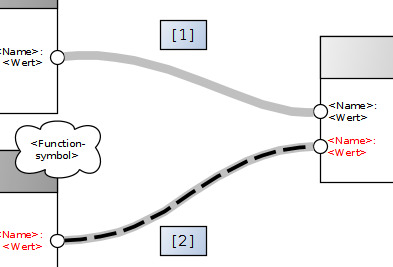
\includegraphics[width=.6\textwidth]{bilder/chapter4/chapter4_3/links.png}
  \caption{Zwei Kanten verbinden vier Input-/Output-Schnittstellen. [1] ist inaktiv während über [2] ein Signal übertragen wird. Man beachte die kurzzeitige Färbung der Input-/Output-Schnittstellen, die auf eine Aktualisierung des Wertes hinweisen.}
  \label{fig:genericlink}
\end{figure}


\paragraph{Kurzbeschreibung} Verbindungen/Kanten sind die Transportwege der Daten, zwischen den einzelnen Knoten. Ähnlich wie ein Leitungen auf einer Platine stellen eine Kante den Transportweg der Signale von einer Output-Schnittstelle zu einer Input-Schnittstelle dar.

\paragraph{Rahmenbedingungen \& Entscheidungen} Jede Verbindung stellt eine eins-zu-eins Beziehung zwischen zwei Schnittstellen dar. Dabei muss sichergestellt werden, dass nur Schnittstellen mit kompatiblen Datentypen verbunden werden können (siehe \hyperref[tab:NFA4]{NFA\#4}). 

\textbf{Aktionen}, die von und in dieser Komponente durchgeführt werden können: 
\begin{itemize}
    \item \textbf{Erstellen} Durch betätigen einer Output-Schnittstelle wird der Erstellungprozess einer Verbindung gestartet und endet mit dem Betätigen einer kompatiblen Input-Schnittstelle oder dem Erstellen eines kompatiblen Funktionsknotens.
    \item \textbf{Löschen} Löscht die Datenübertragung zwischen zwei Schnittstellen und bereinigt die Input-Schnittstelle, in der die Verbindung versinkt.
\end{itemize}

\paragraph{Darstellung} Die Darstellung einer Verbindung ist eine Bézierkurve, die an einer Input-Schnittstelle entsteht und an einer Output-Schnittstelle endet (Abbildung \ref{fig:genericlink}). Sobald Daten durch eine Verbindung fließen, wird eine kurze Animation innerhalb der Bézierkurve gespielt, die den Transfer von Daten entlang der Flußrichtung darstellt (\textbf{[2]}). Der Datentransfer geht verzögerungsfrei vonstatten, ähnlich wie der Transfer von elektrischen Signalen durch Kabel. Deswegen wird die Animation über die ganze Länge der Kurve kurzlebig dargestellt (siehe ''Nähe zur Realität'').

%%%%%%%%%%%%%%%%%%%%%%%%%%%%%%%%%%%%%%%%%%%%%%%%%%%%%%%%%%%%%%%%%%%%%%%%%%%%%%%%%%%%%%%%%%%%%%%%%%%%%%%%%%%%%%%%%%%%%%%%%%

\subsubsection{Sensorknoten}
\begin{figure}[h]
\centering
\begin{subfigure}{.5\textwidth}
  \centering
  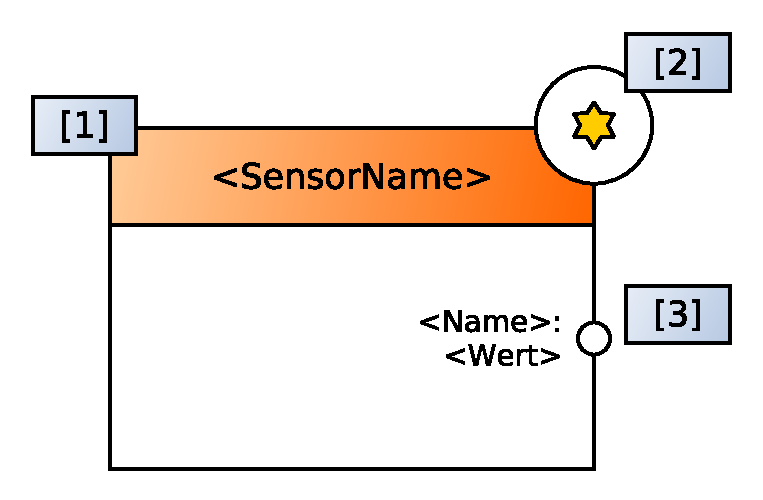
\includegraphics[width=1\linewidth]{bilder/chapter4/chapter4_3/genericsensornode.pdf}
  \caption{}
  \label{fig:genericsensornode}
\end{subfigure}%
\begin{subfigure}{.5\textwidth}
  \centering
  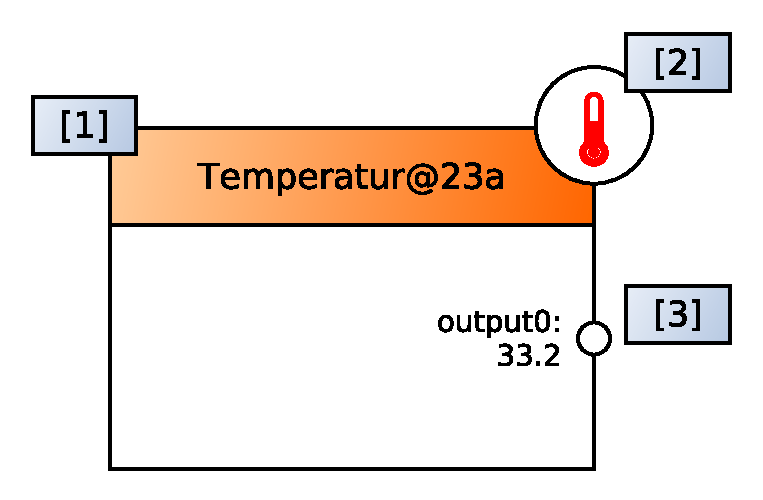
\includegraphics[width=1\linewidth]{bilder/chapter4/chapter4_3/instancesensornode.pdf}
  \caption{}
  \label{fig:sensornodetemperature}
\end{subfigure}
    \caption{Generischer Sensorknoten (a) und Temperatur-Sensorknoten (b)}
    \label{fig:sensornodes}
\end{figure}

\paragraph{Kurzbeschreibung}  Sensorknoten sind die virtuellen Gegenstücke zu den Sensor-cBlocks. Jeder Sensorknoten erzeugt Ereignisse, sobald der Sensor-cBlock eine neue Stichprobe in der Realität entnimmt. Alle Ereignisse werden mit einem Datentyp und dem Messwert als \textit{Payload} über die Output-Schnittstelle an nachfolgende Knoten verteilt. Sobald ein Sensorknoten existiert, sendet er stetig Daten und erlaubt dem Endnutzer kontinuierlich das Verhalten des Graphen zu überprüfen (siehe ''Fehler vorbeugen'' bzw. \hyperref[tab:cognitivedimensions]{fortwährende Evaluation}).

\paragraph{Rahmenbedingungen \& Entscheidungen} Einzelne Sensor-cBlocks können mehrere verschiedene Messwerte auslesen (bspw. Temperatur und Luftfeuchtigkeit im selben Sensor-cBlock). Dem Sensorknoten muss es möglich sein, diese Multifunktionalität abbilden zu können. Es kann sein, dass mehrere Sensor-cBlocks von der gleichen Sorte im selben Prototypen verwendet werden. In diesem Fall, muss es für den Endnutzer möglich sein, die Sensorknoten klar unterscheiden zu können. Gleichzeitig muss es dem es möglich sein leicht, das  physikalische Pendant zu einem virtuellen Sensorknoten zu identifizieren. Ein weiterer Punkt ist die Abtastfrequenz. Sensor-cBlocks liefern Daten in kurz-, lang- oder aperiodischen Frequenzen. Sensorknoten müssen aus diesem Grund darauf achten, synchron mit ihrem physischen Gegenstück, Ereignisse zu erzeugen. Sensorknoten können weder erstellt noch gelöscht werden. Der Status des Sensorknotens, also auch seine Existenz, ist an den Status des Sensor-cBlocks gebunden.

\textbf{Aktionen}, die von und in dieser Komponente durchgeführt werden können: 
\begin{itemize}
    \item \textbf{Identifizieren} durch Betätigen des Knoten-Indikators blinkt die Status LED des korrespondierenden cBlocks. Somit lässt sich sein physisches Pendant identifizieren (siehe ''Nähe zur Realität'').
\end{itemize}

\paragraph{Darstellung} In Abbildung \ref{fig:sensornodes} ist ein generischer Sensorknoten (a) und ein konkreter Temperatur-Sensorknoten (b) dargestellt. Jeder Sensorknoten ist durch eine eindeutige Adresse in der Titelleiste [1] voneinander unterscheidbar. Simultan wird durch \textbf{[2]} der Knotentyp ($\bigcirc$) und seine Rolle ($Thermometer \rightarrow Temperatur$) preisgegeben. \textbf{[3]} sind die Output-Schnittstellen. Jede Art von Messwert eines Sensor-cBlocks erhält einen separaten Output, der den aktuellen Messwert visualisiert. 

%%%%%%%%%%%%%%%%%%%%%%%%%%%%%%%%%%%%%%%%%%%%%%%%%%%%%%%%%%%%%%%%%%%%%%%%%%%%%%%%%%%%%%%%%%%%%%%%%%%%%%%%%%%%%%%%%%%%%%%%%%

\subsubsection{Funktionsknoten}
\begin{figure}[h]
\centering
\begin{subfigure}{.5\textwidth}
  \centering
  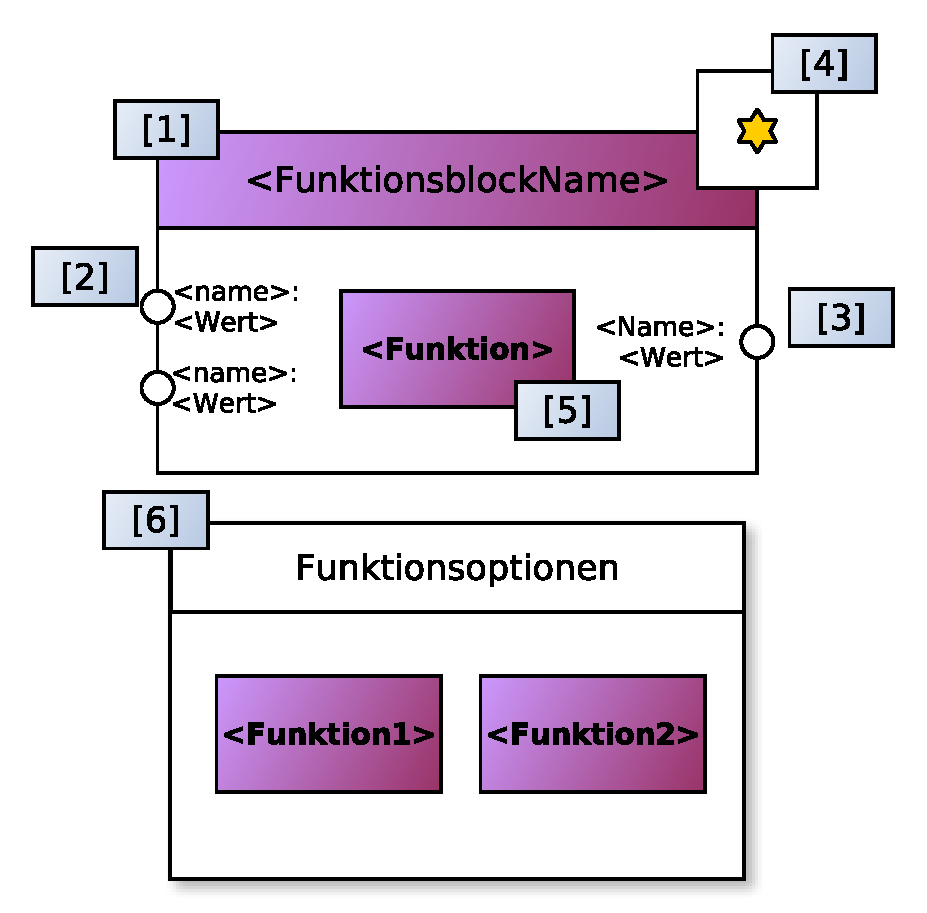
\includegraphics[width=1\linewidth]{bilder/chapter4/chapter4_3/genericfunctionnode.pdf}
  \caption{}
  \label{fig:functionnodesgen}
\end{subfigure}%
\begin{subfigure}{.5\textwidth}
  \centering
  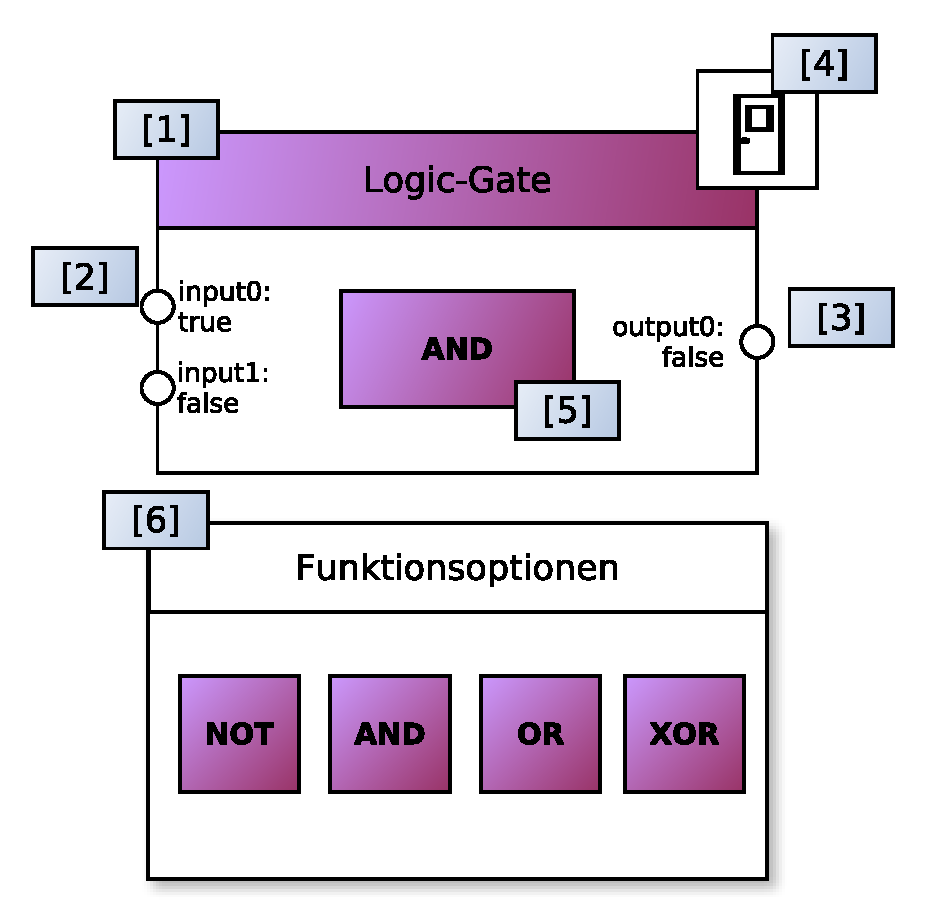
\includegraphics[width=1\linewidth]{bilder/chapter4/chapter4_3/instancegatefunctionnode.pdf}
  \caption{}
  \label{fig:functionnodesgate}
\end{subfigure}
    \caption{Generischer Funktionsknoten (a) und spezifischer Funktionsknoten ''Logisches-Gatter'' (b). Weitere Beispiele für Funktionsknoten im Anhang \ref{anhang:funktionsknoten}}
    \label{fig:functionnodes}
\end{figure}

\paragraph{Kurzbeschreibung} Funktionsknoten sind die Recheneinheiten des Graphen. Der Endnutzer benutzt sie um Signale zu kombinieren und aufzuwerten. Funktionsknoten kommen in einer Bandbreite von Operationsklassen (Logisches-Gatter, Vergleichsoperation, etc.), welche sich an den Datentypen der Ereignisse orientieren (\texttt{String}, \texttt{Number} und \texttt{Boolean}). Jede Operationsart besitzt eine Familie von entsprechenden Operatoren ($\neg, \land,\neq,\geq,$ etc.).

\paragraph{Rahmenbedingungen \& Entscheidungen} Es wurde sich dafür entschieden, Operatoren in Operationsklassen zu bündeln, statt jeder Operation in einen separaten Funktionsknoten auszulagern. Dies soll der Übersicht beitragen und somit das Prototyping beschleunigen (siehe \hyperref[par:movefast]{''Move fast...''}). Des Weiteren lässt sich dadurch die Funktion austauschen ohne den Knoten und somit die Verbindungen austauschen zu müssen (siehe ''vorzeitige Festlegung'' in Tabelle \ref{tab:cognitivedimensions}). Dies beschleunigt das Experimentieren mit verschiedenen Operatoren. Funktionsknoten sind rein virtuell und generisch. Sprich: anders als bei Sensoren/Aktoren können zwei komplett identische Knoten im gleichen Graph existieren.

Die \textbf{Aktionen}, die von und in dieser Komponente durchgeführt werden können: 
\begin{itemize}
    \item \textbf{Löschen} Funktionsknoten begründen ihre Existenz nicht auf ein physisches Pendant, deshalb sind sie anders als Sensor-/Aktorknoten löschbar.
    \item \textbf{Konfigurieren} Die konkrete Funktion wird durch Interagieren mit dem Deskriptor gewählt (siehe Abbildung \ref{fig:functionnodes} und Anhang \ref{anhang:funktionsknoten} für weitere Beispiele)
\end{itemize}

\paragraph{Darstellung}  Der Deskriptor \textbf{[5]} ermöglicht es den momentanen Operator auszulesen. Durch betätigen von [5] wird ein \textit{Modal} \textbf{[6]} geöffnet, indem sich der Operator konfigurieren lässt. In Abbildung \ref{fig:functionnodesgate} ist als Beispiel ein Logikgatter-Funktionsknoten dargestellt. Hier kann der Nutzer die verschiedenen bool'schen Operatoren im laufenden Betrieb konfigurieren und somit das Verhalten des gesamten Graphen zu Laufzeit ändern (siehe '' Move fast...''). Die Schnittstellen \textbf{[2]} und \textbf{[3]} erlauben Parameter und Ergebnis zur Laufzeit auszulesen und Fehler zu überprüfen.

%%%%%%%%%%%%%%%%%%%%%%%%%%%%%%%%%%%%%%%%%%%%%%%%%%%%%%%%%%%%%%%%%%%%%%%%%%%%%%%%%%%%%%%%%%%%%%%%%%%%%%%%%%%%%%%%%%%%%%%%%%

\subsubsection{Aktorknoten}

\begin{figure}[h]
\centering
\begin{subfigure}{.55\textwidth}
  \centering
  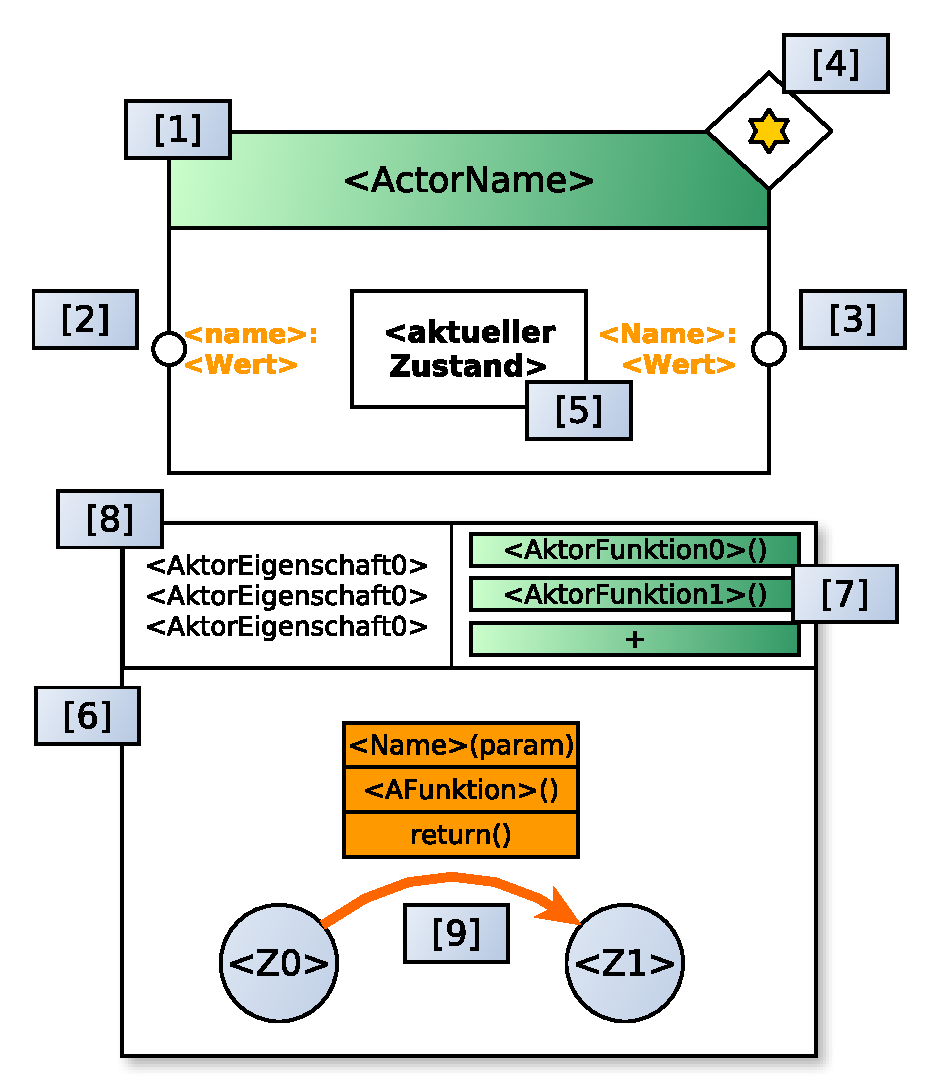
\includegraphics[width=1\linewidth]{bilder/chapter4/chapter4_3/genericactornode.pdf}
  \caption{}
  \label{fig:actorgeneric}
\end{subfigure}%
\begin{subfigure}{.55\textwidth}
  \centering
  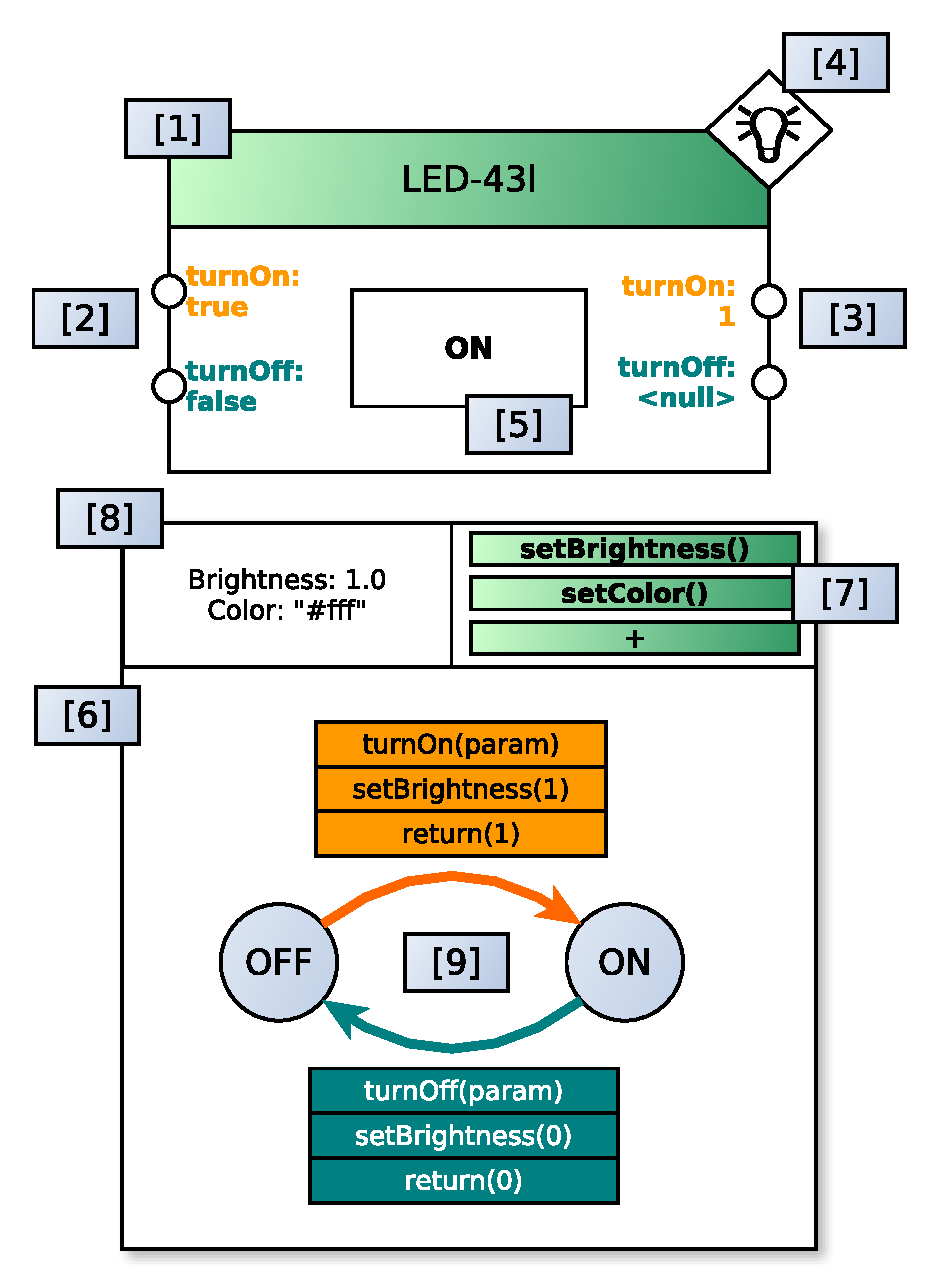
\includegraphics[width=1\linewidth]{bilder/chapter4/chapter4_3/instanceLEDactornode.pdf}
  \caption{}
  \label{fig:actorled}
\end{subfigure}
    \caption{Generischer Aktorblock (a) und spezifischer LED-Aktorblock (b)}
    \label{fig:actornodes}
\end{figure}


\paragraph{Kurzbeschreibung} Aktorknoten sind Sensorknoten ähnlich, indem auch sie, physikalisches Pendants in Form von Aktor-cBlocks besitzen. Durch das Einwirken von Ereignissen verändern Aktorknoten ihren Zustand und steuern somit Aktor-cBlocks. Die Steuerung wird vorgenommen durch eine, vom Endnutzer definierte, \ac{FSM}. Diese \ac{FSM} (siehe Abbildung \ref{fig:actorled} [6]) erlaubt es durch Aktorfunktionen (bspw. \texttt{setColor()}), Aktoreigenschaften (bspw. \texttt{color}) zu verändern und somit die physikalischen Signale des Aktor-cBlocks zu manipulieren. Aktorknoten sind neben dem eigentlichen Graphen die zweite programmierbare Komponente in flowws. Jeder Aktorknoten besitzt eine eingeschränkte Menge von Eigenschaften, die direkt mit den physikalischen Eigenschaften des Aktor-cBlocks korrespondieren. Ein Minimum von Aktorfunktionen wird von flowws vorgegeben.

\paragraph{Rahmenbedingungen \& Entscheidungen} Endbenutzern, denen die mitgelieferten Aktorfunktionen nicht ausreichen, soll es ermöglicht werden, diese nach belieben zu erweitern (siehe ''Grow as you go''). Des Weiteren soll Nutzern es möglich sein, mit den selben Interaktionen, mit denen der Graph modelliert wird, auch die \ac{FSM} zu programmieren (siehe \hyperref[par:fokusbewahren]{''Fokus bewahren''}). Dem Nutzer soll zu jedem Zeitpunkt möglich sein, das Verhalten des Aktors vorauszusagen und nachvollziehen zu können. Aktoren sollen ihren Zustand dem Rest des Graphen mitteilen zu können. Deshalb soll es der Endnutzer in der Lage sein, synthetische Signale zu definieren, die bei einem Zustandswechsel erzeugt werden. Der Status des Aktorknotens ist den Aktor-cBlock gebunden (siehe \hyperref[par:naehezurrealitaet]{''Nähe zur Realität''}). 

\textbf{Aktionen}, die von und in dieser Komponente durchgeführt werden können: 
\begin{itemize}
    \item \textbf{\ac{FSM} erstellen} Zustände, Übergänge und Übergangsfunktionen werden mithilfe der Aktorfunktionen und Aktoreigenschaften vom Endnutzer modelliert
    \item \textbf{Umfang der Aktorfunktionen erweitern} Um den Funktionsumfang zu erweitern können zustandslose Funktionen, welche Aktoreigenschaften modifizieren, vom Endnutzer in Programmcode spezifiziert werden.
\end{itemize}

\paragraph{Darstellung} Der Aktorknoten wird ähnlich wie der Funktionsknoten auf zwei Ebenen dargestellt: der Graphen-Ebene [1] und in Detail-Ebene [8]. Input- [2] und Output-Schnittstellen [3] korrespondieren bei Aktorknoten farblich und namentlich mit den Zustandsübergängen [9] um die Sichtbarkeit des Verhaltens auch außerhalb der Detailansicht zu garantieren (siehe ''Sichtbarkeit'' in Tabelle \ref{tab:cognitivedimensions}). Die momentane Ausprägung der Aktoreigenschaften wird in [8] dargestellt. Die verfügbaren Aktorfunktionen sind in [7] inspizierbar. Die Darstellung der \ac{FSM} in [9] besteht aus Ovalen die Zustände symbolisieren und farbigen Pfeilen die Übergänge definieren. Die Überganglogik wird in einer dreigeteilten Box dargestellt, die sich in Deklaration (Name korrespondiert mit [2] und [3]), Logik (Aktorfunktionen) und Rückgabewert (Der \textit{Payload} des vom Aktor erzeugten Events) aufteilt. Zur Laufzeit ist der momentane Zustand des Aktorknotens ist im Deskriptor [5] ersichtlich.

\subsubsection{Radialmenü}

\begin{figure}[h]
  \centering
  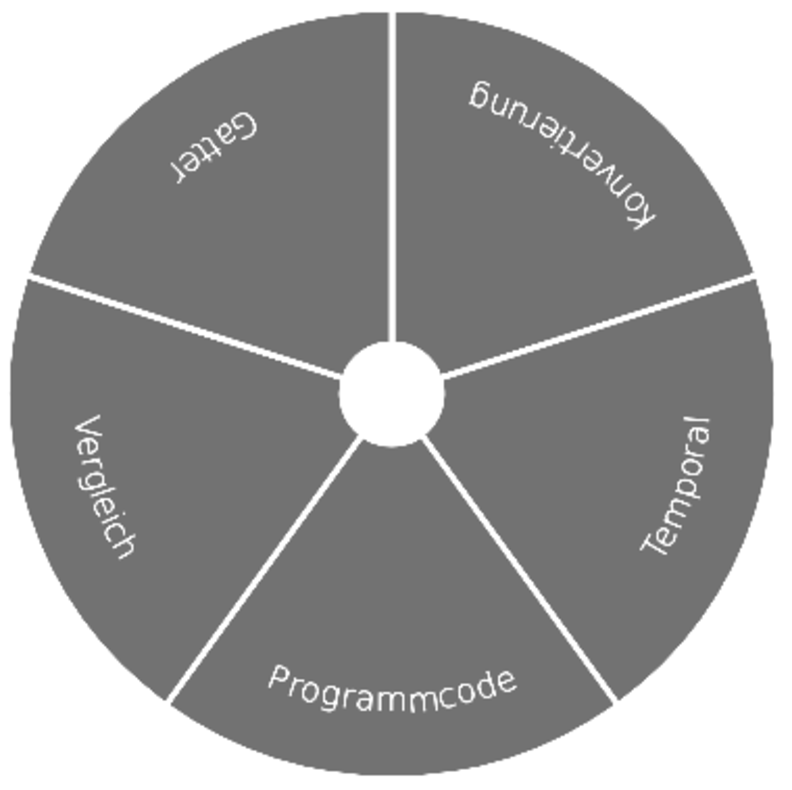
\includegraphics[width=.4\textwidth]{bilder/chapter4/chapter4_3/radialmenu.pdf}
  \caption{Das Radialmenu mit den fünf verschiedenen Operationsklassen aus Kapitel \ref{subsubsec:eventtrans} zur Auswahl}
  \label{fig:radialmenu}
\end{figure}

\paragraph{Kurzbeschreibung} Das Radialmenü ist ein Untermenü, das zu jeder Zeit auf dem Workspace aufgerufen werden kann. Es wird vom Endnutzer verwendet, um Funktionsknoten zu erzeugen.

\paragraph{Rahmenbedingungen \& Entscheidungen} Es wurde sich für ein Radialmenü entschieden, da es im Vergleich zu linearen Menüs schneller zu benutzen ist (siehe ''Move fast...'). Vor allem bei einer vergleichsweise geringen Anzahl von Optionen, die oft verwendet werden müssen (was bei flowws der Fall ist) sind laut \cite{kurtenbach1994user} Radialmenüs besonders effektiv. Das Menü ist kontextsensitiv, d.h. es soll immer nur Operationsklassen von Funktionsknoten zeigen, die zu jenem Zeitpunkt relevant sind. Dies soll zum einen, die Auswahl von inkompatiblen Funktionsknoten verhindern (siehe ''Fehler vorbeugen'') und zum anderen, durch das Verstecken unnötiger Informationen die Arbeitsgeschwindigkeit erhöhen (siehe ''Move fast...'').

Die \textbf{Aktionen}, die von und in dieser Komponente durchgeführt werden können: 
\begin{itemize}
    \item \textbf{Funktionsknoten erstellen} Das Radialmenü ist der einzige Weg für den Nutzer Funktionsknoten zu erstellen. Dazu ruft der Endnutzer das Radialmenü auf und wählt den gewünschten Operationsklassen von Funktionsknoten aus.
\end{itemize}

\paragraph{Darstellung} Das Radialmenü (Abbildung \ref{fig:radialmenu}) ist in fünf Segmente aufgeteilt, bei dem jedes Segment eine Art von Funktionsknoten repräsentiert. Das Radialmenü wird nur nach explizitem Aufruf durch den Endnutzer oder im Kontext von Interaktionen dargestellt und ist sonst nicht sichtbar. 

\subsection{Interaktionen}

flowws benötigt nur eine handvoll Interaktionen, um den Graphen zu erstellen. Aus diesem Grund, werden sich hier auf die drei Wichtigsten beschränkt. %Die meisten Interaktionen sind \textit{Drag-and-Drop} basiert, um die nähe zur Realität zu behalten.

\subsubsection{Verbinden von Knoten}

\begin{figure}[h]
  \centering
  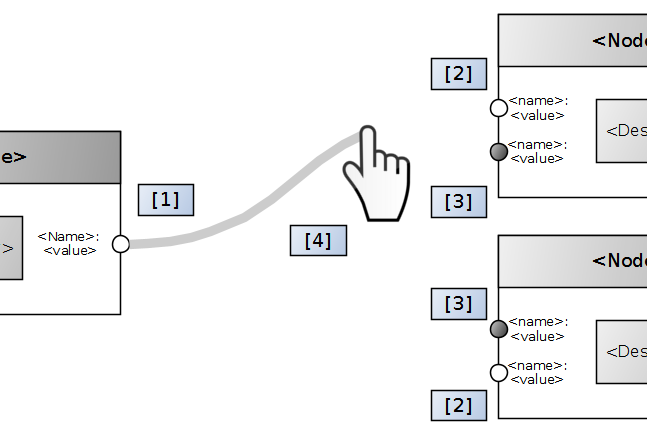
\includegraphics[width=.75\textwidth]{bilder/chapter4/chapter4_3/connectNodes.png}
  \caption{Das Radialmenu mit den fünf verschiedenen Operationsklassen aus Kapitel \ref{subsubsec:eventtrans} zur Auswahl}
  \label{fig:connectNodesInteraction}
\end{figure}
Das Modellieren des Graphen in flowws ist äquivalent mit dem Programmieren von Programmcode. Neben dem Modellieren von \ac{FSM} um das Verhalten von Aktoren zu steuern ist die Hauptarbeit in flowws das Verbinden von Knoten. Das Verbinden von Knoten soll an das Verbinden von Hardware mit Kabeln erinnern (siehe ''Nähe zur Realität''). Aus diesem Grund, wurde sich für eine \textit{Drag-and-Drop}-Interaktion, wie sie in Abbildung \ref{fig:connectNodesInteraction} zu sehen ist entschieden. Hierbei zieht der Endnutzer eine Verbindung von Anfangs-Schnittstelle (a) zu End-Schnittstelle (b). Sobald der Endnutzer diese Interaktion bei (a) beginnt, werden sämtliche potentielle Schnittstellen (b), die mit dem Datentyp von (a) kompatibel sind hervorgehoben. Dadurch soll dem Endnutzer geholfen werden, Fehler zu vermeiden (siehe ''Fehler vorbeugen'').

\subsubsection{Erstellen von Funktionsknoten}

\begin{figure}[h]
  \centering
  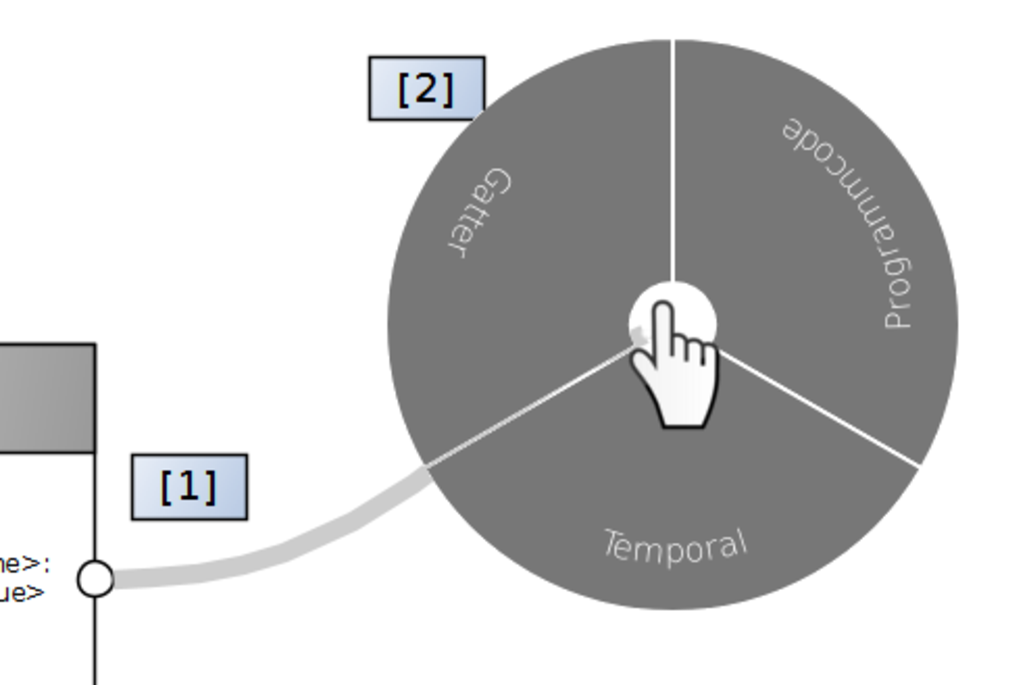
\includegraphics[width=.6\textwidth]{bilder/chapter4/chapter4_3/createNodes.pdf}
  \caption{Das Radialmenu mit den fünf verschiedenen Operationsklassen aus Kapitel \ref{subsubsec:eventtrans} zur Auswahl}
  \label{fig:createNodesInteraction}
\end{figure}
Die Funktionsknoten sind die einzigen Knoten, die in ihrer Existenz nicht an ein physisches Pendant gebunden sind. Aus diesem Grund, werden sie manuell vom Nutzer erstellt und gelöscht. Die Erstellung von Funktionsknoten geschieht mit Hilfe des Radialmenüs. Ein Funktionsblock kann wie in Abbildung \ref{fig:createNodesInteraction} gezeigt auf zwei Weisen erstellt werden: Kontextsensitiv und Kontextunabhängig. \textbf{Kontextunabhängig} können Funktionsknoten auf der ganzen Arbeitsfläche erzeugt werden. Der Benutzer ruft das Radialmenü auf und wählt den gewünschten Knoten aus. \textbf{Kontextsensitiv} ist das Radialmenü Knoten wenn der Endnutzer gerade eine Verbindung erstellt. In diesem Fall, zeigt das Radialmenü nur Optionen an, die für die zu erstellende Verbindung relevant sind. Erstellt der Nutzer bspw. eine Verbindung, die als Quelle den Temperatursensor hat, zeigt das Radialmenü nur Funktionsknoten an, die mit \textit{Number}-Werten (sprich: Temperaturwerten) umgehen können. Für den Endnutzer wird der Erstellungsprozess dadurch übersichtlicher, schneller und weniger fehleranfällig.

\subsubsection{Erstellen von \ac{FSM}}\label{FSMkreieren}


\begin{figure}[h]
  \centering
  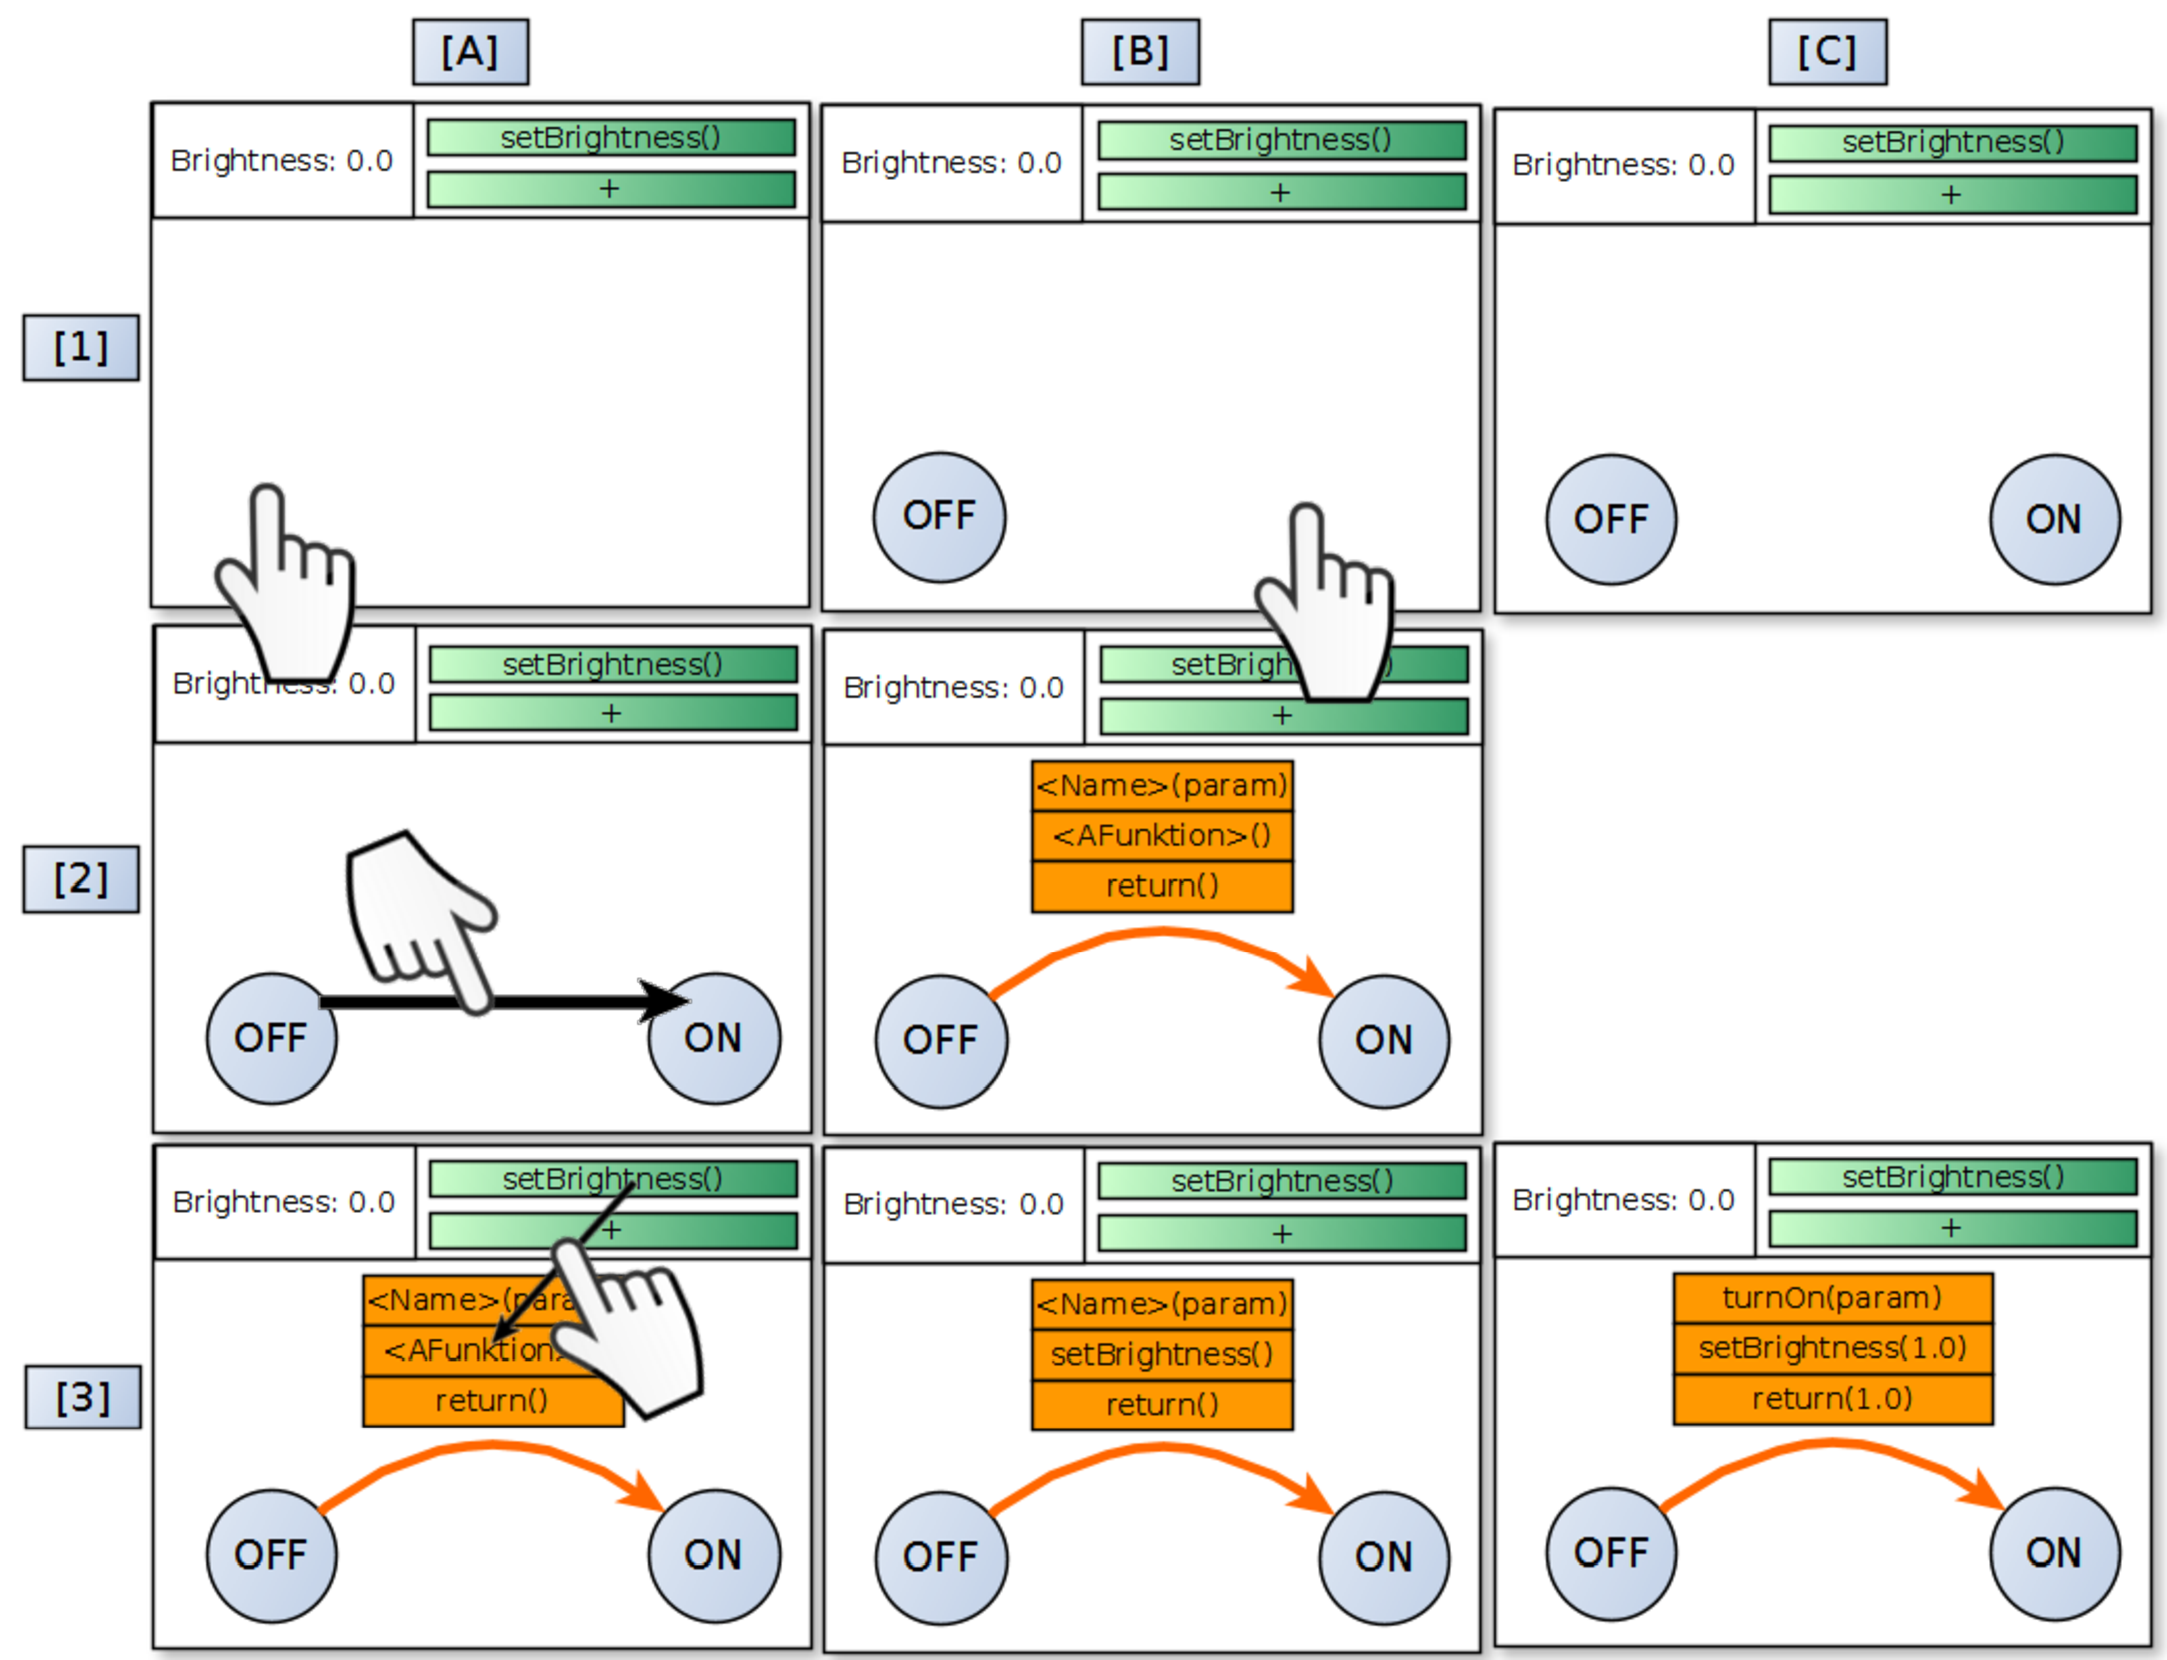
\includegraphics[width=1\textwidth]{bilder/chapter4/chapter4_3/createFsm.pdf}
  \caption{Das Radialmenu mit den fünf verschiedenen Operationsklassen aus Kapitel \ref{subsubsec:eventtrans} zur Auswahl}
  \label{fig:createFSMInteraction}
\end{figure}

Die \ac{FSM} wird in drei Schritten erstellt:
\begin{enumerate}
    \item \textbf{Zustände erstellen und benennen} In [A1] bis [C1] werden durch das Betätigen der Oberfläche Zustände erstellt. Der Endutzer benennt die Zustände und gibt ihnen somit eine symbolischen Bedeutung.
    \item \textbf{Übergänge definieren} Mit einer \textit{Drag-and-Drop}-Interaktion werden vom Endnutzer in [A2] und [B2] die Übergänge zwischen den Zuständen gezogen. Sobald ein valider Übergang entstanden ist bekommt er automatische eine einzigartige Farbe und ein generische Vorlage für die Übergangslogik zugewiesen.
    \item \textbf{Übergangslogik definieren} Die Definition der Übergangslogik geschieht ebenfalls durch \textit{Drag-and-Drop}-Interaktionen. Aktorfunktionen werden hierbei (siehe [A3] bis [C3]) durch den Endnutzer auf die entsprechenden Stellen in der Übergangslogik gezogen. Diese Interaktionen und die manuelle Eingabe der Parameter komplettiert die Programmierung des Aktorknotens.
\end{enumerate}

Es gibt noch weitere Interaktionen die der Endnutzer in flowws durchführen kann, wie das Verwalten von Graphen, das Anordnen der Knoten innerhalb des Graphen oder das Erstellen von Aktorfunktionen. Da diese Interaktionen nicht dazu beitragen Logik für \ac{IoT}-Prototypen zu definieren, werden sie innerhalb dieser Thesis auch nicht behandelt.